%% LyX 2.1.4 created this file.  For more info, see http://www.lyx.org/.
%% Do not edit unless you really know what you are doing.
\documentclass[11pt,english]{article}
\usepackage[T1]{fontenc}
\usepackage[latin9]{inputenc}
\usepackage{geometry}
\geometry{verbose,tmargin=1.25in,bmargin=1.25in,lmargin=1.25in,rmargin=1.25in}
\usepackage{amsmath}
\usepackage{amsthm}
\usepackage{graphicx}
\usepackage{pdflscape}
\usepackage{setspace}
\usepackage{wasysym}
\usepackage[authoryear]{natbib}
\usepackage{pdfpages}
\onehalfspacing

\makeatletter
%%%%%%%%%%%%%%%%%%%%%%%%%%%%%% Textclass specific LaTeX commands.
  \theoremstyle{plain}
  \newtheorem{prop}{\protect\propositionname}
  \theoremstyle{plain}
  \newtheorem{lem}{\protect\lemmaname}

%%%%%%%%%%%%%%%%%%%%%%%%%%%%%% User specified LaTeX commands.
\usepackage{babel}

% set fonts for nicer pdf view
\IfFileExists{lmodern.sty}{\usepackage{lmodern}}{}



\usepackage{babel}
\providecommand{\lemmaname}{Lemma}
  \providecommand{\propositionname}{Proposition}

\date{July 8, 2016 (preliminary draft)}

\makeatother

\usepackage{babel}
  \providecommand{\lemmaname}{Lemma}
  \providecommand{\propositionname}{Proposition}
\usepackage{amssymb}

\begin{document}

\title{Breakable commitments:  \\ present-bias, client protection \\ and bank ownership forms\\ \\ \\ }


\author{Karna Basu \& Jonathan Conning\thanks{Department of Economics, Hunter College \& The Graduate Center, City
University of New York. Email: kbasu@hunter.cuny.edu, jconning@hunter.cuny.edu.
We are grateful to the Roosevelt House Public Policy Institute and
a Small Business Administration research grant for support. For comments
and suggestions, we thank Abhijit Banerjee, Partha Deb, Eric Van Tassel,
and seminar and conference participants at Michigan State University,
IIES Stockholm, Delhi School of Economics, Queens College, Indian
School of Business, Hunter College, Florida Atlantic University, CIDE-ThReD
Conference on Development Theory, and NEUDC. Kwabena Donkor provided
excellent research assistance.}}
\maketitle
\begin{abstract}
When do financial intermediaries provide the `commitment services' that can help present-biased consumers  stick to  long-term  responsible savings accumulation and/or debt management plans? When do banks instead aim to opportunistically profit by pandering to their clients' self-control problems or, the related question, by how much is financial trade reduced by the fear that such opportunism might take place? We study a simple workhorse model of saving \textit{cum} lending and refinance to   hyperbolic discounters to understand a consumer protection problem that survives even when
consumers are fully informed and sophisticated. The consumer would like
to commit her future selves to  a balanced multi-period path of saving accumulation \textit{cum} debt repayment via a commitment contract with a bank, but her future
selves can be tempted to take on new debt obligations and/or raid savings by subsequent contract renegotiation offers.   Investor-owned banks may find it especially costly to credibly commit to not engage in 
 such opportunistic `exploitation'  as  bank ex-post profits evidently increase by doing so. In markets with sophisticated consumers this can lead to lower ex-ante consumer welfare or bank profits and lost trade. In such situations bank principals may make costly strategic adjustments to bank ownership/governance forms to expand the credible commitment (or renegotiation-proof ) contracts and hence capturable profits. This forms the basis for a  theory of commercial non-profits and endogenous client protection similar to \cite{hansmann_ownership_1996}  but on new behavioral micro-foundations. Non-profit and `hybrid'  bank ownership forms (e.g. with  social investors to temper bank profit objectives) may be able to offer commitment services at lower cost as limitations on the distribution of profits weakens banks' incentive to renegotiate
contracts but the equilibrium set of  contract and ownership forms is endogenous and will depend on whether the market is competitive or concentrated and with elements of the legal environment such as the enforceability of exclusive contracts. The model provides a framework for studying the historical evolution of ownership forms in consumer banking, microfinance, and mortgage and payday lending and for thinking about frequently heard calls for consumer protection against excessive refinancing and `overindebtedness'  in these sectors. JEL Codes: O16, D03,
D18
 

\end{abstract}

\section{Introduction}



Hyperbolic discounters -- consumers with present-biased preferences -- are those who struggle to stick to  their long-term asset accumulation or debt management plans and for that reason may benefit from
the `commitment services'  or  designed restrictions that a financial intermediary may build into multi-period financial contracts.   Long-term consumption smoothing goals are more likely to be achieved where customers can enlist financial intermediaries to act as partners in resisting  temptations to raid savings and/or   increase debt in ways that could undermine  responsible long-term plans. The properties of \textit{costlessly}-enforced optimal
commitment banking contracts have been examined in several theoretical papers
(\cite{laibson_golden_1997}) and a number of randomized controlled trials and other empirical studies have   found quite large impacts from introducing new commitment service savings products (see for example \cite{Thaler_Benartzi_2004}, \cite{ashraf_tying_2006} and the studies mentioned in the survey by \cite{bryan_commitment_2010}). 

The assumption of costless commitment services is hard to sustain. Commitments can be broken and the same person that at first demanded a commitment
contract from a bank may  later want to renegotiate its terms. A bank's ex-post profits may well be increased by pandering to such demands.   For example, a present-biased consumer who takes out a loan that  promises to balance repayments and expected consumption across future periods may
at a later period find themselves unable to resist the temptation to refinance to take out an expensive (but at this later date attractive)\  additional consumption   loan that drives up present consumption but wrecks earlier laid consumption smoothing plans.    

This type of problem raises obvious consumer protection concerns in the case of naive or partially naive present-biased consumers
as these are consumers who, by definition, do not understand how their own future preferences will evolve to make them vulnerable to such opportunistic exploitation by a bank. In the absence of consumer protection a  bank could attempt to lure customers into contracts that it knows can  be later renegotiated for additional profit.  
 
In the case of sophisticated present-biased consumers consumer protection issues also arise but take the less obvious and  harder to measure form of lost or reduced financial trade. \ Sophisticated consumers anticipate the possibility of opportunistic contract renegotiation and therefore will be cautious to minimize their vulnerability by insisting on renegotiation-proof contracts that must be endogenously enforced. But  imposing  any such additional constraints can only reduce the feasible financial contract space, reducing gains of trade and therefore lowering bank profits and/or consumer welfare or lost trade.
\ The practical result in either case will be equilibria with less than optimal consumption smoothing  with consumes saving `too little' and/or borrowing `too much' (in the estimation of their earlier period selves) in some periods compared to situations where full-commitment contracts could be costlessly offered.

Concerns over excessive refinancing and `over-indebtedness' have been raised repeatedly in recent years in both the developed and the developing world.    On the eve of the mortgage banking crisis in 2007, over 70 percent of new subprime mortgage loans were refinances
of existing mortgages and approximately 84 percent of these were `cash out' refinances (\cite{demyanyk_understanding_2011}).  In the market for payday loans the  concern of many economists and regulatory observers is not so much that fees are high for one-time short-term loans (typical cost is 15\% of the amount borrowed on a 2 week loan) but rather that over 80 percent of payday loans are in fact `rolled over' or renewed rather than paid off, incurring new fees each time resulting in very high  total loan costs and  placing many people into  very difficult debt management situations (\cite{DeYoung_2015}.\footnote{Approximately half payday loans are rolled over in sequences lasting 7 or more turns}   

Similar concerns have been raised in microfinance markets in developing countries but in such markets where  government  consumer protection laws are weak to non-existent, the issues
take on an interesting extra dimension.
To state our hypothesis briefly and bluntly:  microfinance markets around the world have been dominated by a mix of mission-driven and commercial non-profits and  `hybrid' firms -- for example for-profit firms  partly or entirely owned and controlled by not-for-profit foundations or governments (\cite{conning_microfinance_2011,cull_microfinance_2009}). We argue that this is because, compared to investor-led for-profit firms hybrid and non-profit firms can make more credible commitments to not engage in the type of opportunism described above, because their incentive to do so is muted by the fact that they cannot easily distribute any profits. This is a variation on Henry Hansmann's theory of commercial non-profits but set on new behavioral micro-foundations that we will model explicitly below. In the early stages of new microfinance markets one or more non-profit firms will dominate and successfully provide the commitment services in savings and credit contracts.  However as market competition intensifies the capturable advantages of strategic non-profit status are diminished and this can lead to a `commercialization' stage and the conversion of many commercial from non-profit to for-profit form. This will be associated with a rise of of the type of consumer protection issues identified above and  concomitant collapse of borrower and saver discipline. This helps make sense of the string of repayment crises in places as far flung as Morocco, Bosnia, Nicaragua, and Andra Pradesh in India where previously very successful microfinance markets followed similar trajectories 
   

 In this paper we view the provision of commitment as an important
element of consumer protection in banking. Our goal is to provide a simple dynamic framework
for analyzing real-world settings where commitment is demanded but
cannot be credibly provided at zero cost. We work with a quite general three-period consumption smoothing model for a sophisticated present-biased consumer with quasi-hyperbolic preferences that allows for saving(repayment) or borrowing(dissaving) in each period. In each contracting scenario the consumer's period zero self (henceforth `Zero self')\ has a bias for present consumption but wants to smooth future consumption across periods one and two.  They correctly 
anticipate that their later period-one `One self' will have a change of preferences that  will lead them to want to `raid savings' and/or take on new debt to drive up period one consumption at the expense of period two consumption, thereby undoing One self's early intent to balance consumption across the two periods. In every case the equilibrium contract will be the subgame Perfect
Nash equilibrium of a game where Zero self chooses a contract  first anticipating One self's reactions, possibly limited by the Bank's exogenously or endogenously enforced commitment to agree to not renegotiate with One-self.   

In the first part of the paper we characterize the contracts associated with three broad scenarios: (1)\ \textbf{`Own smoothing' contracts }where the consumer saves on their own without a bank that might offer commitment services; (2)\ \textbf{Full-commitment contracts} where we  assume the Zero self consumer can enter into multi-period contract that binds their One self to not renegotiate the contract terms under the assumption that this bank commitment can be costlessly enforced; and (3) \textbf{renegotiation-proof contracts} where the zero self consumer can enter into a multi-period  contract to  bind their One self to not renegotiate the contract terms but where the bank's commitment must be endogenously enforced by making sure that bank's ex-post profits from breaking their commitment fall short of any direct renegotiation costs to the bank summarized by a parameter $\kappa$. We describe the terms of renegotiation-proof contracts and the distribution of gains to trade between bank and consumer and how these are parameterized by $\kappa.$ At high enough values the bank can credibly commit to not profit from renegotiation and the first-best costless full-commitment contract can be achieved.  In the second part of the paper, described below, we explore how a bank might make costly strategic changes to its bank ownership and governance structures as another way to credibly commit to not renegotiate.    

We are able to provide quite complete characterizations of optimal contracting scenarios under the assumption of monopoly or competition in the market for period-zero banking contracts with or  without the assumption of enforceable exclusive contracts in later periods. We can provide exact closed-form solutions for contract terms for  CRRA utility functions for most of these cases including renegotiation-proof contracts when $\kappa=0$.  For the   $\kappa>0 $ cases where closed form solutions cannot be directly obtained we can  nonetheless characterize some important contract properties and solve for contracts numerically. Separately we also characterize the terms of the contract that would be offered to a naive present-biased consumer by a bank that would strategically renegotiate the contract.  

 





      

 

 



With sophisticated hyperbolic discounters, the bank wishes it could
credibly commit to not renegotiate in the future. Its choice of governance
and ownership structures may help it do so. A nonprofit firm, for
example, faces legal restrictions on its enjoyment of earnings. So,
if the bank operates as a nonprofit, it can demonstrate to the consumer
that it has less to gain from future renegotiation. This improves
its ability to commit to a commitment contract, which allows it to
extract more surplus from the consumer. Whether it chooses to adopt
nonprofit status depends on the extent to which legal restrictions
improve its ability to commit while protecting its ability to enjoy
the additional surplus extracted through commitment. That nonprofit
firms may survive even in the absence of motivated agents or asymmetric
information is, to the best of our knowledge, a novel result.

Our model considers nonprofits more broadly than in the above example,
and analyzes governance choices across consumer types and market settings.
A monopolist bank prefers to operate as a nonprofit if consumers need
relatively small adjustments to their consumption. In competitive
markets, exclusivity plays an important role--if contracts are exclusive,
firms operate as nonprofits; otherwise, for-profits dominate.



Banks, under both monopoly and competition, may explore commercial
nonprofit status as a mechanism to more credibly commit to not opportunistically
exploiting the weaknesses of its sophisticated time-inconsistent clients.
By operating as a nonprofit (or more broadly as a `hybrid' bank),
the bank agrees to face legal or governance restrictions on how any
profits generated from any such opportunistic renegotiation can be
distributed and enjoyed. The bank can now credibly convince the sophisticated
consumer that it will be less likely to renegotiate the contract in
the future. This allows the bank to offer the consumer an initial
contract that maintains the restrictions on future consumption patterns
that the consumer demands, raising the contracting surplus and therefore
how much can be ultimately extracted by the bank's stakeholders.

A firm's decision about whether to adopt nonprofit status rests on
a trade-off. As a non-profit, the firm has an opportunity to extract
greater surplus from the consumer (by providing commitment), but now
faces restrictions on the ability of managers and shareholders to
enjoy this surplus. In the case of monopoly, the bank will adopt nonprofit
status if the following is true: non-profit restrictions should be
sufficiently severe that the bank is able to extract more surplus
from the consumer, but should not be so severe that it is unable to
enjoy the surplus. We show how the details of the trade-off depend
on the governance choices available to the bank and the consumer's
reservation outcomes.

This trade-off is also sensitive to market structure. Under competition,
a lender's ability to provide effective commitment through non-profit
status depends on the exclusivity of contracts. When long-term contracts
can be made exclusive, the trade-off disappears and all active firms
function as non-profits. This is because of the zero-profit condition--since
firms do not make profits anyway, there is nothing to lose from switching
to non-profit status. On the other hand, there are profits to be gained--if
all other firms are for-profit, a firm could make positive profits
by offering superior commitment as a non-profit (this is valuable
even if its enjoyment of these profits is limited).

When contracts are not exclusive, commitment generated through non-profit
status becomes impossible to achieve. Since non-profit firms would
make zero profits anyway, each firm has an incentive to switch to
for-profit status so it can take advantage of the opportunity to re-finance
\textit{other} banks' loans. As a result, for-profit firms must be
active in equilibrium, and their presence will eliminate the possibility
of non-profit commitment.

This can partly explain a key difference between traditional non-profit
microfinance, which is rigid, and say commercial credit card lending
which offers refinancing flexibility (credit card punishments gain
salience because they are\textit{ less} strict, not more). 

The model is indeed stylized and limited to one of many mechanisms,
but we argue that it makes a number of compelling points relevant
to ongoing policy debates and is able to explain some stylized facts.



\subsection{Context and Related Literature}


\subsubsection{Commitment as Consumer Protection}

Problems of consumer protection are typically analyzed through two
channels: naive or uneducated consumers and their failure to correctly
anticipate fees and punishments (see \citet{gabaix_shrouded_2006},
\citet{armstrong_consumer_2012}, and \citet{akerlof_phishing_2015}
for related arguments), and bank's moral hazard (see \citet{dewatripont_prudential_1999}
and \citet{oak_only_2010}). We argue that, given the growing evidence
of time-inconsistent preferences,\footnote{See, for example, \citet{laibson_debt_2003}, \citet{ashraf_tying_2006},
\citet{gugerty_you_2007}, and \citet{tanaka_risk_2010}.} a bank's ability to provide credible commitment should also fall
under this umbrella--sometimes consumers \textit{want} punishments
or fees to limit renegotiation.

In recent years, especially in light of crises in consumer credit
markets, there has been renewed emphasis on consumer protection and
better governance and regulation in banking.\footnote{In the US, the Consumer Financial Protection Bureau was set up in
2011 under the Dodd--Frank Wall Street Reform and Consumer Protection
Act. In India, the far-reaching Micro Finance Institutions (Development
and Regulation) Bill of 2012 was designed to increase government oversight
of MFIs in response to the credit crisis in the state of Andhra Pradesh,
and the perception that lax consumer protection and aggressive lending
practices had led to rising over-indebtedness and stress.} One particular outcome of concern has been borrower over-indebtedness,
an issue that has been at the center of recent microfinance repayment
crises in places as far-flung as Morocco, Bosnia, Nicaragua and India,
as well as the 2008 mortgage lending crisis in the United States.
In each of these cases the issue of refinancing or the taking of loans
from multiple lenders emerges. For example, by value, more than two-thirds
of the subprime mortgage loans outstanding in 2008 were made up of
refinanced loans (\citet{demyanyk_understanding_2011}).

Journalistic and scholarly analyses of such situations, including
the recent mortgage crisis in the United States, have often framed
the issues as problems of consumer protection, suggesting that many
lenders designed products to purposefully take advantage of borrowers
who have limited financial literacy skills and are naive about their
self-control problems. Informed by such interpretations, new regulations
introduced in the wake of these crises have swung toward restricting
the terms of allowable contracts, for example by setting maximum interest
rates, and the use of coercive loan recovery methods.

We place consumers' struggles with intertemporal self-control issues
at the center of the analysis, but argue that borrowers may be more
sophisticated in their understanding of their own time-inconsistency
than is often assumed. From this perspective, `predatory lending'
is not primarily about tricking naive borrowers into paying more than
they signed up for with hidden penalties or misleading interest rates
quotes, but about offering excessive flexibility and refinancing of
financial contracts in ways that limit or undermine the commitments
to long term consumption and debt management paths that borrowers
themselves may be attempting to put in place.\footnote{\citet{bond_predatory_2009} discuss evidence of predatory lending
in the context of mortgages.}

A sophisticated hyperbolic discounter understands that his `future
selves' will attempt to take out new loans on top of old ones, or
renegotiate the terms of existing loans to further defer debt repayment.
If she is a saver, she will try to withdraw more rapidly in the future
than she would have liked, or will deposit less than ideal. That such
consumers should be and are willing to pay for commitment has been
demonstrated in several theoretical and empirical papers (for examples
of commitment, see \citet{ashraf_tying_2006}, \citet{carrillo_promises_2008},
\citet{bryan_commitment_2010}, \citet{fischer_repayment_2010}, \citet{banerjee_poor_2011},
and \citet{basu_hyperbolic_2011}). By entering into a contract that
commits them to a specific time-path of repayments or deposits, the
consumer attempts to ensure that future selves will not skew consumption
patterns to privilege instant gratification in the following periods.
Viewed this light, fees and punishments for failing to adhere to a
schedule are not inherently undesirable to the consumer--for sophisticated
hyperbolic discounters, threats of punishment can indeed serve as
useful commitment devices. 

Nevertheless, the fact that consumers value commitment does not automatically
imply that firms will provide it in equilibrium. In fact, there remains
an open question about whether markets can be relied upon to supply
commitment. The key consideration in this paper is the following:
if a hyperbolic discounter is willing to pay to commit her future
selves, her future selves are willing to pay to undo this commitment.
Here, a bank that promises to be rigid and is then flexible could
be seen as hurting, rather than helping, the consumer. We take seriously
the bank's ex-post considerations and derive conditions under which
it would renegotiate.

In this sense, our paper complements some others that demonstrate
how commitment can be undone in related settings. \citet{gottlieb_competition_2008}
shows how competition leads to inefficient outcomes in immediate rewards
goods. \citet{heidhues_exploiting_2010} study the mistakes of partially
naive borrowers in competitive credit markets. \citet{mendez_predatory_2012}
analyzes predatory lending with naive consumers. Our emphasis is on
the terms of any generic banking contract, analyzed broadly: under
both competition and monopoly (the latter being particularly relevant
to informal banking in developing economies), for both sophisticated
an naive consumers, and for multiple governance and ownership structures.


\subsubsection{Commercial Nonprofits}

The idea that firm ownership might be strategically chosen to solve
or ameliorate `contract failure' problems dates back at least to \citet{arrow_uncertainty_1963}
and is one that has been articulated most clearly in the work of Henry
Hansmann (1996). Hansmann
argued that in markets where the quality of a product or service might
be difficult to verify, clients may rationally fear that investor-led
firms will be tempted to opportunistically skimp on the quality of
a promised product or service, or reveal a hidden fee, and this can
greatly reduce or even eliminate contracting. In such circumstances
becoming a `commercial non-profit' may be a costly but necessary way
to commit the firm to not act opportunistically, hence enabling trade. 

Hansmann gives as a primary historical example the development of
consumer saving, lending and insurance products in the United States
and Europe. Life insurance in the United States for example has until
quite recently always been dominated by mutuals. Rate payers could
not trust investor-led firms to not act opportunistically by, for
example, increasing premiums or by skimping or reneging on death benefit
payouts. Mutuals on the other hand had little incentive to cheat clients
to increase shareholder dividends as the clients themselves are the
only shareholders. Mutuals therefore enjoyed a distinct competitive
advantage until sufficient state regulatory capacity developed.

In the present analysis we begin by following Hansmann in defining
nonprofits by the legal restrictions faced by them, setting aside
other ways (such as motivation) in which they might be different from
for-profit firms.\footnote{Hence we abstract away from other considerations for nonprofits, as
in \citet{besley_competition_2005}, \citet{mcintosh_competition_2005},
and \citet{guha_micro-finance_2013}. Nonetheless our modeling framework
can be adapted to include these considerations and is the focus of
related work.} In this view \textquotedbl{}{[}a{]} nonprofit organization is, in
essence, an organization that is barred from distributing its net
earnings, if any, to individuals who exercise control over it, such
as members, officers, directors, or trustees.\textquotedblright \footnote{In practice, nonprofit firms also enjoy certain benefits that are
denied to for-profit firms (see, for example, Cohen, 2015 {[}FIND
CITATION{]}). But for the purposes of Hansmann's (and our) argument,
it is the \textit{restrictions}, not benefits, that generate improved
outcomes.} \citet{glaeser_not-for-profit_2001} have formalized Hansmann's central
argument to show that when a firm cannot commit to maintaining high
quality, it might choose to operate as a commercial nonprofit rather
than as an investor-led for-profit in order to credibly signal that
it has weaker incentives to cheat the consumer on aspects of unobserved
product quality. As Hansmann describes it, firm ownership form adapts
endogenously as a ``crude form of consumer protection'' in unregulated
emerging markets where asymmetric information problems are rife. \citet{bubb_consumer_2013}
modify this model so that the non-contractible quality issue is on
hidden penalties, which are incurred with certainty by some borrowers.
All of these models are built rely on some form of asymmetric information
or contract verification problem.

A contribution of our paper is to argue that a theory of ownership
form can be built on behavioral micro-foundations even in environments
with no asymmetric information and with sophisticated forward-looking
agents. We believe this is an important element for understanding
the development of consumer finance in developed countries historically
as well as the current shape of microfinance today where non-profit
and `hybrid' forms still dominate the sector in most developing countries
(\citet{cull_microfinance_2009,conning_microfinance_2011}). Hybrid
ownership forms include the many microfinance firms that, though technically
incorporated as for-profit financial service providers, are in fact
dominated by boards where, by design, social investors or client representatives
exert substantial governance control. Hybrid forms such as these would
appear to confer many of the benefits of non-profit status (specifically,
credible commitment to consumer protection) with fewer of the costs
(in particular, unlike a pure non-profit they can and do issue stock
to outside investors although usually in a manner that does not lead
to challenge control).


\subsubsection{Market Structure and Governance Choice}

Commenting upon a major microfinance crisis in the state of Andhra
Pradesh in India, veteran microfinance analyst Elizabeth Rhyne (\citet{rhyne_microfinance:_2011})
describes the build up of ``rising debt stress among possibly tens
of thousands of clients, brought on by explosive growth of microfinance
organizations . . .\textquotedblright{} fueled by the rapid inflow
of directed private lending and new equity investors who, because
they ``paid dearly for shares in {[}newly privatized{]} MFIs . .
. needed fast growth to make their investments pay off.\textquotedblright{} 

Her analysis, like that of many others, ultimately lays the blame
on ``poor governance structures.\textquotedblright{} In her view,
Indian MFIs might have avoided their problems and followed the model
of leading microfinance organizations in other countries like Mibanco
(Peru) and Bancosol (Bolivia) which ``were commercialized with a
mix of owners including the original non-governmental organization
(NGO), international social investors (including development banks),
and some local shareholders. The NGOs kept the focus on the mission,
while the international social investors contributed a commercial
orientation, also tempered by social mission.'' These are the types
of hybrid ownership forms, along with nonprofit firms, that we argue
can provide surplus building consumer protection through a reduced
incentive to renegotiate. However, as our model demonstrates, these
governance choices are highly dependent on market structure, and nonprofits
may survive better under monopoly than under competition.





\section{The Model: Setup}


\subsection{Consumers and their selves}

There are three periods, $t\in\left\{ 0,1,2\right\} $. In any period
$t$ the consumer's instantaneous utility is given by a CRRA function
defined over all nonnegative consumption 
\begin{equation}
u\left(c_{t}\right)=\begin{cases}
\frac{c^{1-\rho}}{1-\rho} & \mbox{if \ensuremath{\rho>0\mbox{ and }\rho\neq1}}\\
ln\left(c\right) & \mbox{if \ensuremath{\rho=1}}
\end{cases}
\end{equation}
Given a consumption stream $C_{t}=\left(c_{t},c_{t+1},...,c_{2}\right)$,
the period-$t$ self's discounted utility is: 
\begin{equation}
U_{t}\left(C_{t}\right)\equiv u\left(c_{t}\right)+\beta\sum\limits _{i=t+1}^{2}\delta^{i-t}u\left(c_{i}\right)
\end{equation}
This describes quasi-hyperbolic preferences (\cite{laibson_golden_1997}), with a hyperbolic discount
factor $\beta\in(0,1]$.
In any period, the individual places greater relative weight on present-period
gratification than her earlier selves would have liked. The consumer
could be sophisticated or naive about the time-inconsistency of his
preferences (\citet{odonoghue_choice_2001}).

As the consumer's preferences are time-inconsistent it will be useful to distinguish between the consumer's different selves. We refer to the  period-zero consumer as the `Zero-self' and her  period-one incarnation as her `One-self'. 


\subsubsection{Consumption smoothing and the problem of  self-control}



Zero-self begins with claims to an arbitrary
income stream $Y^0=\left(y_{0},y_{1},y_{2}\right)$ over the three
periods. Her objective is to rearrange this into a utility maximizing
consumption stream. In the absence of  formal banking services she must rely
on informal saving or  borrowing, if available. 

The amount of consumption smoothing the consumer is likely to  achieve under autarky will in general fall short of that that might be achievable with well functioning formal financial trade for a variety of reasons. If
her income is back-heavy, borrowing constraints may limit her ability
to smooth consumption, and in the absence of credit she must consume
her income as it arrives.  If her income is front-heavy, the consumer may be able to construct a somewhat smoothed autarky
stream with own savings strategies but technological and/or institutional restrictions  may limit the returns to saving \(   r\) to low or negative rates, with insecurity of storing cash at home being one obvious
explanation.


  \begin{figure}[p!]
    \centering
    \vspace*{-2cm}
    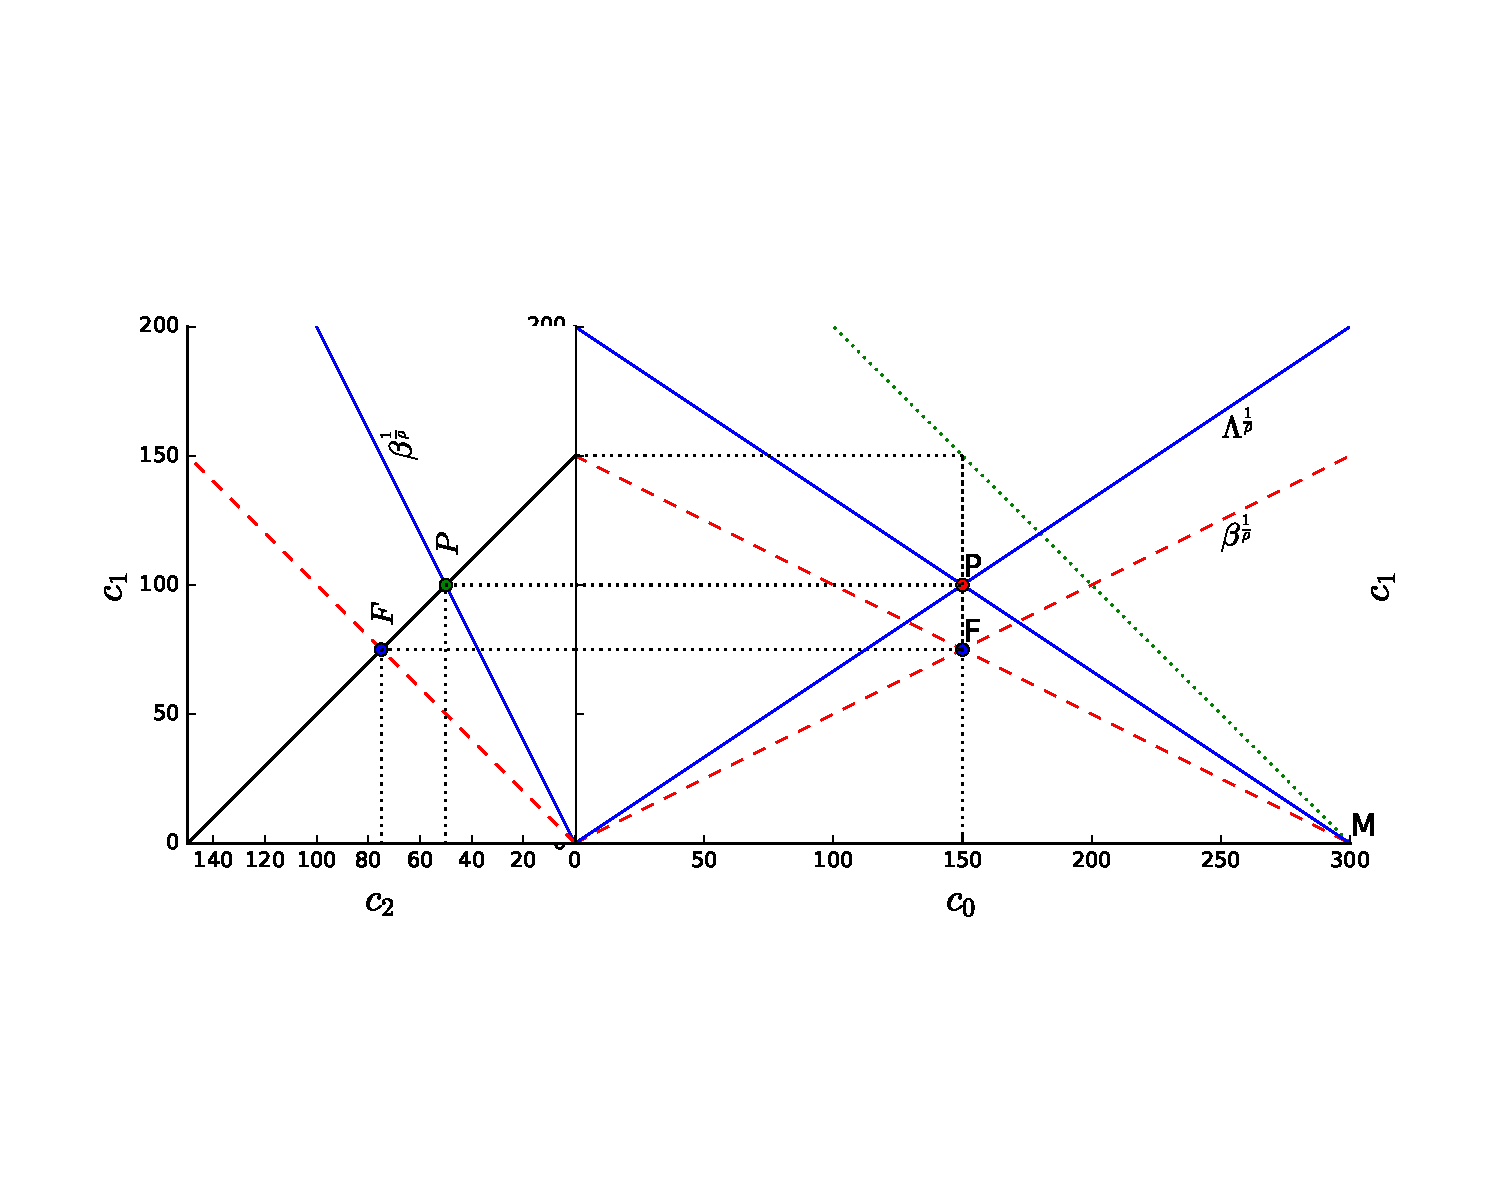
\includegraphics[angle=90,width=\paperwidth]{fig_twopanel.pdf}
    \caption{\label{fig:twoquad}Self-control and the demand for commitment}
  \end{figure}


\begin{figure}
  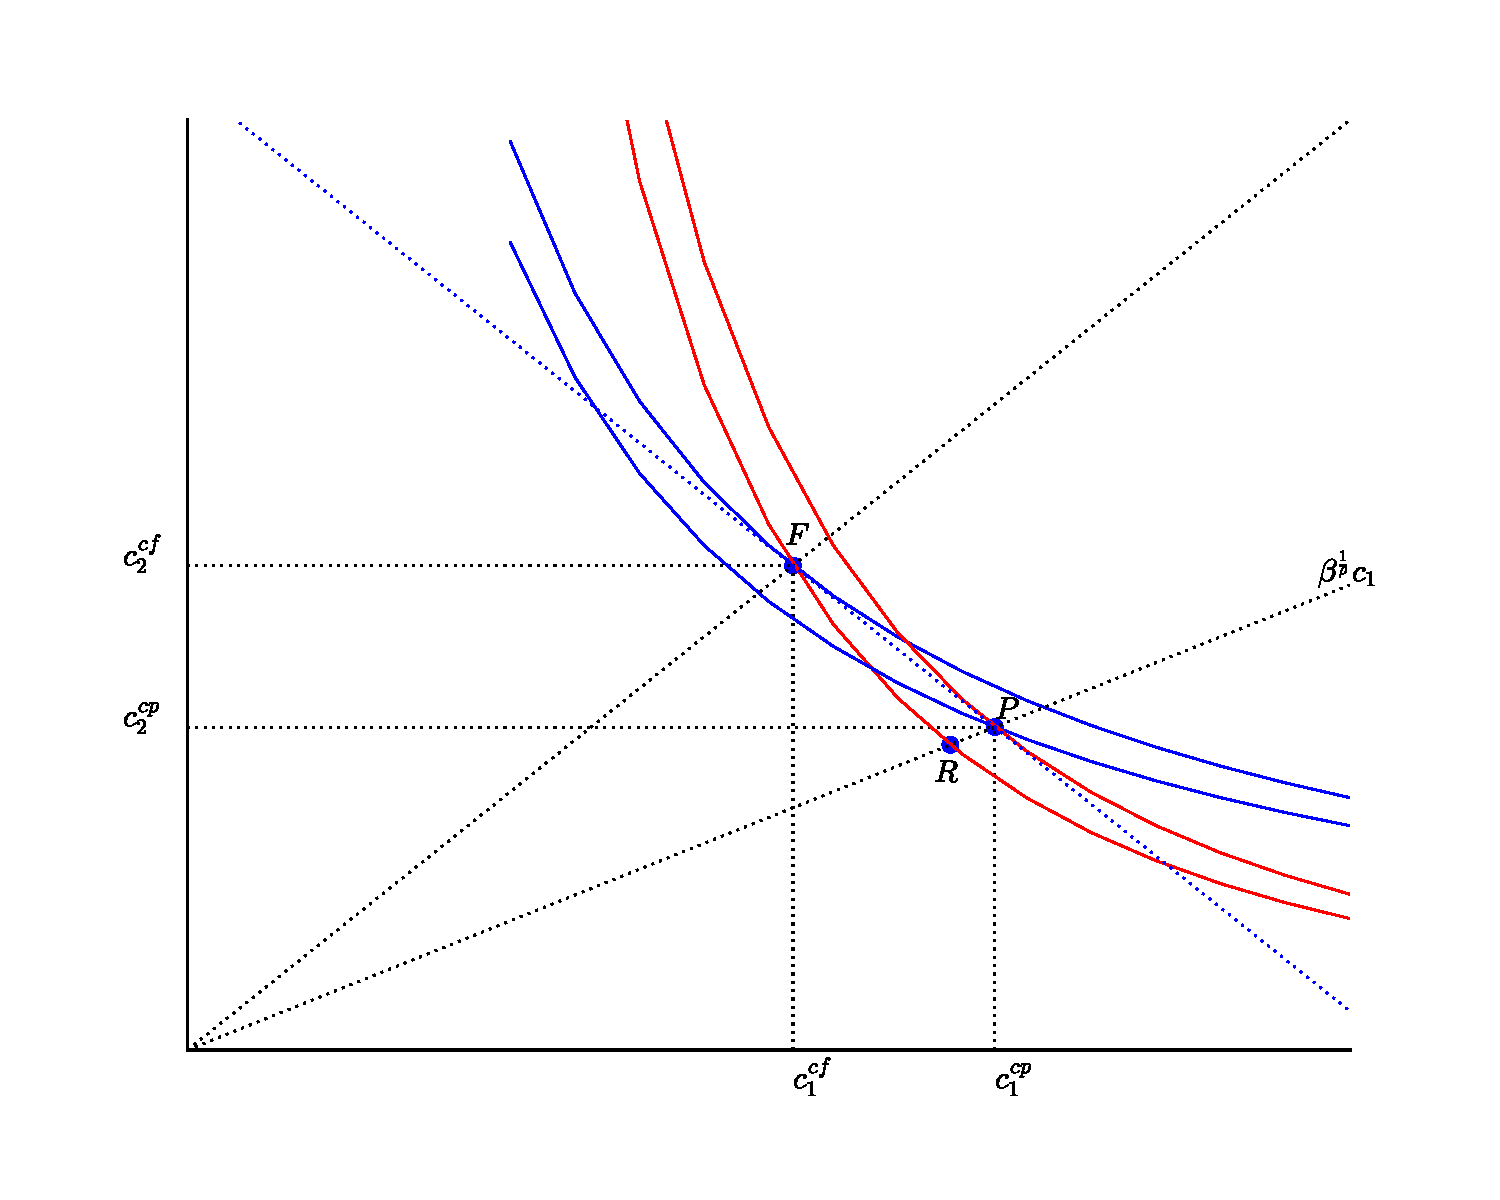
\includegraphics[width=\textwidth]{fig_selfcontrol.pdf}
  \caption{\label{fig:c1c2}Period 1 recontracting}
\end{figure}

 More  central to our analysis, however, is  that
 a consumer with time-inconsistent
preferences generally cannot trust her later selves to not disrupt her preferred long-term 
consumption plans.  Zero  would like to control her later selves ability to change consumption plans but in the absence of such self-control she will find herself locked into a  strategic contracting game with  her latter self which will limit her to less than optimal consumption plans.  

To highlight the consequences of the absence of  self-control problem most clearly let us temporarily assume the consumer has access to informal borrowing or saving at constant competitive interest rate \(  r\). First we establish the benchmark case where Zero can contract for an ideal optimal consumption smoothing contract as if she faced no self control problem. This is  a standard utility maximization problem subject to an  inter-temporal budget constraint
(or, same thing, subject to a financial intermediary's zero-profit condition):\begin{displaymath}
 \max_{C^0} U_0(C^{0})
\end{displaymath}
\begin{displaymath}
\Pi^0(C^0,Y^0)=\sum\limits _{i=t}^{2} \frac{\left(y_{t}-c_{t}\right)}{\left(1+r}\right)^i} \geq 0
\end{displaymath}
The familiar first-order necessary conditions are: \begin{displaymath}
u'\left(c_{0}\right)=\beta \delta (1+r) u'\left(c_{1}\right)=\beta \delta^2 (1+r)^2u'\left(c_{2}\right)
\end{displaymath}
 These equations plus the binding budget constraint allow us to solve for $C^0$. Conceptually the equilibrium contract is given by the  tangency where the consumer has reached the highest feasible iso-utility surface  touching the hyper-plane defined by the budget. A 3D graphical analysis is cumbersome but the problem can be understood better with 2D contour projections.         

With CRRA utility these three equations can be rewritten:
\begin{equation} 
c_1=[\beta\delta(1+r)]^\frac{1}{\rho}c_{0}   \label{eq:FOCc0c1}
\end{equation}
\begin{equation}
c_2=[\delta^{2}(1+r)^{2}]^\frac{1}{\rho}c_{1} \label{eq:FOCc1c2}
\end{equation} 
This last equation and the budget constraint can be combined to give:
\begin{equation}
c_1=\frac{\sum y -c_0}{1+[\delta (1+r)]^\frac{2}{\rho}} \label{eq:budgetplus}
\end{equation}

Equations \ref{eq:FOCc0c1} and \ref{eq:budgetplus} allow us to solve for $c_0$ and then  the remaining periods.  The term $\delta (1+r)$ enters each expression above and essentially `tilts' consumption to be more generally rising or falling over time as  $\delta \gtreqless 1/(1+r)$.  As this general tilt is not essential to the analysis below (however the degree of present-bias $\beta$ will be)  we shall without loss of generality impose the assumption that  \(\delta=\frac{1}{1+r}\) to unclutter the math. The above equations then become simply

\begin{equation}
c_1=\beta^\frac{1}{\rho}c_{0} \text{,   }
c_2=c_{1} \text{ and }
c_1 = \frac{\sum y-c_0}{2}  
\end{equation}

In words: Zero self wants to indulge her present bias to tilt consumption toward period zero consumption but to then allocate consumption evenly across the remaining two periods. From the above a closed form solution for \(C_{0}\) is easily found: 

\begin{equation}
c_0^{0F} = \frac{\sum y}{1+2\beta^\frac{1}{\rho}} \\ \label{eq:CF}
\end{equation}

\begin{equation*}
c_1^{0F} = c_2^{0F} = \beta^\frac{1}{\rho}c_0^{0F}
\end{equation*}

These relationships and the Zero's preferred contract solution be seen in the two-panel diagram of Figure \ref{fig:twoquad},  drawn for a consumer with $\beta = 0.5$ and $\rho=1$ and a present value of income \(y=300\) spread over the three periods (we are assuming \(r=0\)).\footnote{These parameter values are chosen for expositional simplicity. In particular  $\rho=1$ will imply that period zero consumption will  be the same under full commitment as in the case where self-control is not possible, This simplifies certain graphical interpretation of the self-control problem but the analysis readily extends to other values.} 
The right hand panel is drawn in $c_0-c_1$ contract space.  Points along the ray OF satisfy first-order equation \ref{eq:FOCc0c1} while points along the ray MF satisfy  the second tangency equation \ref{eq:FOCc1c2}  and  the budget line (i.e. they satisfy equation  \ref{eq:budgetplus}).   The intersection at F identifies the coordinates $(c_0^F,c_1^F)$ of Zero's preferred contract, also given by equation \ref{eq:CF}. We've labeled this with subscript F to indicate it's essential similarity to the full-commitment contract that might be offered by a competitive bank.\footnote{This will be exactly the same full-commitment contract that a competitive bank intermediary would be led to offer if they faced an opportunity cost of funds  $r$ identical to what we have assumed here for the informal economy (normalized to $r=0$ for convenience only)\..   However since it is realistic to assume these rates will not be the same and  that in practice consumers in the informal economy may face lower, possibly negative rates of return on informal savings and higher rates (and/or constrained access to loans.} The left hand panel depicts the situation in $c_1-c_2$ space of the sliced plane  at $c_0=c_0^F$). Details of this last diagram can be seen (now rotated 90 degrees)  in Figure \ref{fig:c1c2}.  Points along ray OF satisfy the Euler equation \ref{eq:FOCc1c2}, while points along the line passing through DF satisfy the period 1 budget $c_1+c_2=\sum y - c_0^$ where $c_0=c_o^F$ in this case. Point F at the intersection of these lines identifies the coordinates $(c_1^F,c_2^F).$

For these  parameter values Zero's preferred contract
is $(c_0^F,c_1^F,c_2^F)=(150, 75, 75)$. Whether the consumer saves or borrows in each period  depends on the value of her income in that period relative to their chosen consumption level.  If the consumer's total income of 300 were divided evenly as $Y_{0}=(100, 100, 100)$ then this  preferred consumption plan would be achieved by borrowing $c_0-y_0=50$ in period 0 and repaying  25 in each of periods 1 and 2 (recall \(r=0)\). If the  stream were instead $Y_{0}=(200, 50, 50)$ the same consumption plan could now be constructed by saving  50 in period 0 to be evenly allocated to raise consumption in periods 1 and 2. In both cases we have assumed that One self cannot alter the consumption plan.  

Let us now analyze what happens when  the self-control problem  cannot be solved and  One self cannot be stopped from attempting to recontract.  One-self will want to indulge her new present-bias and therefore `over-consume' in period 1  relative to what Zero self had intended. We may think of this as One self      `raiding savings'  or `piling on new debt' in period 1 at the expense of  period 2 consumption. 
Figure \ref{fig:c1c2} (which provides extra detail on a rotated version of the left panel of Figure \ref{fig:twoquad}) illustrates the problem. Assume for a moment that the consumer had (naively as it will turn out) accepted the contract \(C_0^F\) in period zero. At the start of period 1 this contract satisfies Zero self's optimality condition $u'(c_1^F)=u'(c_2^F)$ but from the standpoint of One self's preferences involves too little period 1 consumption as $u'(c_1^{0F})\geq \beta u'(c_2^{0F})$. At point F, Zero self's indifference curve is tangent to the budget line but One self's indifference curve is steeper than the budget line. One self can   gain by recontracting to any feasible tangency point along the $c_2=\beta^\frac{1}{\rho}c_1$ ray, above where that indifference curve cuts the line and and   below the budget line.\footnote{ We have assumed that One self has access to finance at the same interest rate $r$.  Figure \ref{fig:c1c2} also assumes $\rho=1$.  When $\rho \neq 1$ point P will not lie exactly on the budget line defined by $c_0+c_1=\sum y - c_o^F$ as $c_o^F \neq c_o^P$ but the analysis of Figure \ref{fig:twoquad} is readily adapted.}  A sophisticated    Zero self consumer anticipates such recontracting and how it would lower their inter-temporal utility. They can do not better  to limit the damage than to accept the contract at P (as any other contract that satisfies the budget constraint would be recontracted to P anyways).  This subgame-perfect renegotiation-proof contract will involve less net saving (or same thing, more net debt) in period 1 than Zero self would prefer ($u'(c_1^{P})<  u'(c_2^{P})$) and a lower Zero self welfare.


A sophisticated hyperbolic discounter who fully anticipates her own future
change of preferences finds herself locked into a strategic game with her latter self to try to limit the damage.\footnote{A naive hyperbolic discounter, on the other hand, may believe she
can achieve optimal utility though this will not be realized. See below.} This has the structure of a Stackelberg game with Zero self moving to choose a contract first in anticipation of One self's best recontracting best response. }   
To see this  consider One self's best response in any subgame defined by Zero self's choice of contract \(C^{0}=(c_0^0, c_1^0,c_2^0)  \). \ One self can either accept the remaining consumption plan  $(c_1^0,c_2^0)$ or exchange it for a new contract to solve
\begin{displaymath}
 \max_{c_1,c_2}  u(c_1)+\beta u(c_2)
\end{displaymath}       

\begin{displaymath}
 s.t. c_1+c_2 \leq c_1^0 +c_2^0
\end{displaymath}       

Since Zero self's budget constraint must bind at an optimum (otherwise consumption and utility could be increased) the period 1 budget can be rewritten
\begin{equation}
 c_1+c_2 \leq \sum y -c_0^0
\end{equation}
From this it is  clear that all that One self needs to react to is zero self's choice of period zero consumption $c_0^0^$ which establishes the net remaining resources to be divided between period 1 and 2.  From the earlier equation \ref{eq:budgetplus} we know Zero self would like each extra unit of savings that it passes forward into period 1 to be, on the margin, equally shared between period 1 and period 2 consumption (i.e. slope of the line through MF is $\frac{dc_1}{dc_0}=-\frac{1}{2}$ when $\delta=\frac{1}{1+r}$).

One self on the other hand wants to set $c_2=\beta^\frac{1}{\rho}c_1$ which substituted into a binding period one budget can be solved to give a best response function to Zero self's choice of period 0 consumption:
\begin{equation}
c_1^{1}(c_0^0)=\frac{\sum y - c_0^0}{1+\beta^\frac{1}{\rho}}  \label{eq:react1}
\end{equation}
\begin{equation}
c_2^{1}(c_0^0)=\beta^\frac{1}{\rho}\frac{\sum y - c_0^0}{1+\beta^\frac{1}{\rho}}
\end{equation}
One's reaction function is given by the line passing through MP in the left quadrant of Figure \ref{fig:twoquad}.  As  long as $\beta\leq 1$, for any given level of consumption in period 0,  One self wants to consume more in period 1 and less in period 2 relative to what One self would prefer.

The sophisticated Zero self anticipates her future self's reaction and therefore chooses $c_0^0$ strategically to solve:
\begin{displaymath}
\max_{c_0} u(c_0)+\beta[u(c_1^{1}(c_0)+u(c_2^{1}(c_{0})]\\  
\end{displaymath}
subject to 
 \begin{displaymath}
 c_0+ c_1^{1}(c_0)+ c_2^{1}(c_0)= \sum y
\end{displaymath}
Using the fact that $c_2=\beta^\frac{1}{\rho}c_1$ and other substitutions the first-order condition for this problem can be written:
\begin{equation*}
u'(c_0)=\Lambda u'(c_1)
\end{equation*}
\begin{equation}
c_1=\Lambda^\frac{1}{\rho}c_0 \label{eq:LambdaC0}
\end{equation}
where 
\begin{equation}
\Lambda=\frac{(\beta+\beta^\frac{1}{\rho})}{1+\beta^\frac{1}{\rho}}
\end{equation}
Analogously to the case of the classic Stackelberg Cournot duopoly game our Zero self wants to choose the consumption contract  on the highest iso-utility surface along her opponent's reaction function. This point is given  by contract \(P \text{ }\)which satisfies both equation \ref{eq:react1} (the line through MP) and equation \ref{eq:LambdaC0} (the line through OP). These two equations can be solved to give a closed-form solution to the optimal contract in the absence of self-control \begin{equation}
c_0^P = \frac{\sum y}{1+\Lambda^\frac{1}{\rho}(1+\beta^\frac{1}{\rho})} 
\end{equation}
with $c_1^P=\Lambda^\frac{1}{\rho}c_0^P$ and c_2^P=\beta^\frac{1}{\rho} \Lambda^\frac{1}{\rho}c_0^P$. As can be seen in Figure \ref{fig:c1c2}, Zero self has little choice but to accommodate to the fact One self will grab a fraction of any of the consumption resources that Zero self would have liked to have made available or period 2 consumption. For our earlier parameterization $\beta=0.5$ and $\rho=1$ the best contract in the absence of self-control will be $C_0^P=(150, 100, 50) $ which offers considerably less consumption smoothing in later periods compared to the contract with self-control $C_0^F=(150, 75, 75) $.  If the consumer has income stream $Y_0=(100, 100, 100)$ then we can think of the consumer with self-control as sticking to a balanced repayment program to keep consumption steady in the last two periods. Compared to this the consumer without self-control postpones rolls over rather than repays the portion of the debt that they would have paid off in period one, lowering period 2 consumption. If the consumer had had an income stream $Y_0=(200, 50, 50)$ then a consumer without self-control can be viewed as raiding   savings in period that an otherwise identical consumer with self-control would have earmarked to boost period 2 consumption. Put differently, `solving'   the self control problem  leads consumers to save more/borrow less in period 1 and consume more in period 2. 

For the diagram exposition we  focused on the special case where $\rho=1$ which implies an elasticity of inter-temporal substitution of $\sigma=\frac{1}{\rho}=1$.  This in turn implies that period zero consumption will be the same under self-control or its absence. It is possible to show that $c_0^P>c_0^F$ or $c_0^P<c_0^F$ as $\rho<1$ or $\rho>1$ respectively.  That is to say the consumer may raise or lower period 0 consumption as part of their effort to indirectly control their latter self's choices.  However the amount by which $c_0^P$ will differ from $c_0^F$ is  negligible to very small compared to the differences in period 1 and period 2 consumption for all parameters values in the range $0\leq \beta \leq 1$ and $0\leq \rho \leq \infty $. In practical terms this means that in the absence of self-control the Zero self can do very   little but to accommodate to One self's preferences in establishing the balance of consumption between period 1 and period 2. This relative lack of power in turn leads to the demand for commitment services from a financial intermediary, the topic which we turn to next.    



\subsection{Banks}

The Zero-self consumer has the option of contracting with one or many
risk-neutral banks, depending on the market structure. Each bank has
access to funds that can be withdrawn from other investments at an
interest rate $r$. 

For expositional simplicity we assume that $r=0$ and that the consumer's
discount factor is $\delta=\frac{1}{1+r}$ (so $\delta=1$). This will imply that at an optimum the Zero-self would like flat consumption, or \(c_{1}=c_2\).  This without loss of generality as equivalent derivations
for arbitrary $r$ and $\delta$ can be constructed in the same manner. Working with this special case greatly de-clutters many of the math formulas that follow without subtracting any fundamental insight.

 Any financial contract between the consumer and the bank can be thought
of as the consumer trading claims to income stream $Y_{0}$ in exchange for
a consumption path $C_{0}$. A financial contract involves a period
0 loan if the exchange is such that $c_{0}>y_{0}$ and a period 0 savings contract
if $c_{0}<y_{0}$. 

The bank can perfectly enforce feasible repayment plans, so the net
present value of its remaining profit stream in period t is given
by: 
\begin{equation}
\Pi_{t}\left(C_{t};Y_{t}\right)=\sum\limits _{i=t}^{2}\left(y_{t}-c_{t}\right)
\end{equation}


The bank will participate and offer a contract if and only if it can earn non-negative
profits.
If the contract were to be renegotiated in period 1, the bank would
incur a non-monetary cost, $\kappa>0$, which could be interpreted
to include a concern for reputation or some other impact on the social
preferences of its owners.\footnote{The bank could incur additional monetary costs as well. However, we
assume these to be 0 as they can be netted out and do not affect the
analysis in any important way (we also separately analyze the $\kappa=0$
case for comparison.)} The bank fully knows the borrowers preferences and can tailor the
contract by borrower type.


\section{Full-Commitment}

We first derive properties of the benchmark equilibrium `full-commitment'
contract in the absence of renegotiation possibilities before describing
how the contract would change when the consumer anticipates the possibility
of contract renegotiation between his later-period self and the bank.


\subsection{Monopolist Bank}

A monopolist bank aims to rearrange consumption in a way that extracts
maximum surplus from the consumer while satisfying her participation
constraint (PC), i.e. leaving her no worse off than in autarky. The
bank solves the following problem:

\begin{align}
\max_{C_0} & \; \Pi_{0}\left(C_{0};Y_{0}\right)\nonumber \\
s.t. & \; U_{0}\left(C_{0}\right)\geq U_{0}^{A}\label{eq:PC}
\end{align}


The first-order conditions  are familiar and intuitive--they require
that the discounted marginal utilities of consumption be equalized
across periods:
\begin{equation}
u'\left(c_{0}\right)=\beta u'\left(c_{1}\right)=\beta u'\left(c_{2}\right)
\end{equation}


This, combined with the Zero-self's participation constraint (which must bind at a monopoly optimum)
yields the solution, denoted $C_{0}^{m,fc}$ (the superscript is for
`monopoly, full commitment') and corresponding bank profits $\Pi_{0}\left(C_{0}^{m,fc};Y_{0}\right)$
. Closed form solutions for the CRRA case appear as appendix equations \ref{eq:c-mf} and \ref{eq:pi-mf}, respectively.\footnote{Explicit closed-form solutions for this and continuing contract terms are in the appendix.} 

A number of observations can be made. Any contract satisfies $c_{0}>c_{1}=c_{2}$
to satisfy period 0's desire for instant gratification and her desire
to equalize consumption across all future periods. Whether the contract
in each period is interpreted as a loan (or dissaving) or savings (or repayment) will depend on the position
of the consumer's initial autarky bundle relative to this point.

The terms of the optimal monopoly contract, and hence also the level of bank
profits achieved is dependent on the consumer's autarky utility. $C_{0}^{m,fc}$
rises and profits fall with $U_{0}^{A}$  . The bank makes non-negative profits. 


It is worth noting how commitment enters implicitly in such a contract--the
bank agrees to maintain a particular relationship between consumption
in periods 1 and 2 that the consumer, given her time-inconsistency,
would otherwise have been unable to sustain.


\subsection{Perfectly Competitive Banks}

Consider now a situation where multiple banks compete to offer the
consumer contracts in period 0. We continue to first describe the
full-commitment equilibrium contracts that arise in markets where
due to aspects of the legal and institutional environment contracts
can be simply assumed to remain \emph{non-renegotiable} and \emph{exclusive}.
By exclusive we mean situations where once a competitively determined
contract is established other banks can be prevented from establishing
new or additional contracts with the customer and his future selves
in any period. We will then relax both these assumptions one by one,
analyzing the need for renegotiation-proof contracts and the firms'
strategic choice to possibly operate as a non-profit first when contracts
remain exclusive and then in non-exclusive contracting contexts where
other banks cannot be prevented from offering customers new contracts
in later periods.

Banks compete to attract consumers subject to a bank's participation
(zero-profit) constraint (BPC). The equilibrium contract satisfies:

\begin{align}
\underset{C_{0}}{\mbox{\ensuremath{max }}} & U_{0}\left(C_{0}\right)\nonumber \\
s.t. & \Pi_{0}\left(C_{0};Y_{0}\right)\geq0\label{eq:BPC}
\end{align}


A contract will be accepted if it leaves the consumer with at least
the discounted utility she receives in autarky. The first-order conditions
are exactly as under the monopoly case. Substituting these into the
zero-profit constraint allows us to easily solve for the full-commitment
competitive equilibrium contract. We denote the solution $C_{0}^{c,fc}$
(equation \ref{eq:c-cf}).

As in the monopoly case the contract panders to period 0 self's present
bias and offers smooth flat consumption in later periods. But unlike
under monopoly, where $C_{0}^{m,fc}$ is as low as possible, under
competition consumption in every period is relatively higher--$C_{0}^{c,fc}$
is raised to the point where it satisfies $\sum_{t=0}^{2}c_{t}^{c,fc}=y$.
As a result, banks get zero profits and the consumer perfectly smoothes
consumption and gets utility $U_{0}^{*}$. The equilibrium contract
is not dependent on the consumer's autarky utility.


\subsection{Naivete vs Sophistication}

A hyperbolic discounter may be considered sophisticated (being aware
in period 0 that her period 1 self will discount the future by $\beta$)
or naive (incorrectly believing that in period 1 she will not discount
the future). Given a particular autarky utility, the above solutions
do not depend on any assumptions of sophistication or naivete. But
it should be noted that in cases where the consumer self-saves in
autarky, the naif may believe she can do better than she actually
does. In such cases, $U_{0}^{A}$ is weakly higher for the naif than
for the identical sophisticated agent. This leaves the competitive
equilibrium unchanged, but under monopoly will result in a tighter
participation constraint, resulting in greater consumption for the
consumer. So the naif's failure to correctly assess her future could
leave her better off than otherwise.


\section{The Renegotiation Problem}

As explained above, contracts in part provide commitment. As a result,
with sophisticated hyperbolic discounters who value such commitment,
bank profits too can be thought of as deriving in part from satisfying
the customer's demand for commitment. The bank can charge for helping
the customer stick to preferred savings accumulation/loan repayment
plans that deliver balanced consumption across periods 1 and 2. However,
this is conditional on its ability to credibly promise to not pander
to the customers' later self's demands to raid savings or take out
new loans that might disrupt those plans. Since balanced consumption
is not optimal from period 1's perspective, when that period arrives
she would like to renegotiate the contract. And since this renegotiation
may be profitable to the bank, this needs to be taken seriously.


\subsection{Monopoly}

\begin{figure}

\includegraphics[width=\textwidth]{fig_monopoly.pdf}
\caption{\label{fig:renegotiation}The monopoly renegotiation problem}

\end{figure}


Figure \ref{fig:renegotiation}, which is drawn in $c_{1}-c_{2}$
space, illustrates the problem by showing how a monopolist could profit
by reneging on a consumption smoothing contract \textit{ex-post},
how a sophisticate anticipates this possibility, and therefore why
a monopolist might earn more by taking costly actions to try to make
their commitment to a contract more credible \textit{ex-ante}. Point
$F$ is the balanced consumption $\left(c_{1},c_{2}\right)$ component
of the monopolist's optimal contract. At this point period 0's participation
constraint (\ref{eq:PC}) is satisfied. The flatter of the two indifference
curves passing through point $F$ represents the consumer's period
0 self's preference, $u\left(c_{1}\right)+u\left(c_{2}\right)$, which
gives equal weight to period 1 and period 2 consumption while line
NF can be interpreted as the isoprofit line associated with the monopolist's
maximum profits from period 1 forward.

The demand for commitment arises from the fact that the period 0 self
understands that as soon as period 1 rolls around her preferences
will change and the period 1 self will accept renegotiated contract
offers to raise period 1 consumption even if this comes at the cost
of period 2 consumption and period 0's discounted utility.\footnote{Measured in period 1 utils, the period 0 self values consumption bundle
$(c_{1},c_{2})$ as $u(c_{1})+u(c_{2})$ whereas period 1 self values
the same bundle as $u(c_{1})+\beta u(c_{2})$.} Hence at contract point $F$ in the the period 1 self's preferences
are represented by the steeper indifference curve and at that point
we have $u^{\prime}\left(c_{1}\right)>\beta u^{\prime}\left(c_{2}\right)$. 

The figure illustrates how a bank can increase could opportunistically
'exploit' a consumer whose earlier self had agreed to $F$ by offering
new consumption stream $R$ in exchange. This would raise period 1
consumption by 'raiding savings' (or taking out a new loan) of a customer
with the effect of lowering the net savings (or increasing the net
debt) passed into period 2 compared to what the customer had earlier
demanded.

The contract at R would be designed to raise period 1 self's discounted
utility ever so slightly while raising the monopolist to the higher
value isoprofit line $RQ$. A sophisticated present-biased customer
will however anticipate the possibility of renegotiations of this
sort and will only agree therefore to renegotiation-proof contracts
that are invulnerable to such exploits. Requiring that contracts are
renegotiation-proof adds constraints to the contract design problem
so the monopolists' profits can only fall relative to the full-commitment
benchmark where we simply assumed it could costlessly commit itself
to no renegotiations. The customer, who was already pushed against
their autarky reservation utility, is no worse off than before.

More formally, consider the renegotiation problem that arises in period
1. A customer who has agreed to contract $C_{0}$ in period 0 enters
period 1 with claims to the remaining consumption stream $C_{1}$.
This determines the new reservation utility. If profitable to the
bank, the optimal renegotiated contract will be chosen in period 1
to solve:
\begin{align}
\underset{C_{1}^{m,r}}{max} & \Pi_{1}\left(C_{1}^{m,r};C_{1}\right)\nonumber \\
s.t. & U_{1}\left(C_{1}^{r}\right)\geq U_{1}\left(C_{1}\right)\label{eq:pc-r}
\end{align}


The bank offers $C_{1}^{m,r}\left(C_{1}\right)\equiv\left(c_{1}^{m,r}\left(C_{1}\right),c_{2}^{m,r}\left(C_{1}\right)\right)$
(equation \ref{eq:c-r}) to replace\footnote{The bank swaps net income stream $\left(y_{1}-c_{1},y_{2}-c_{2}\right)$
for $(y_{1}-c_{1}^{r},y_{2}-c_{2}^{r})$.} the contractually agreed $C_{1}$. Since the first-order conditions
imply $u^{\prime}\left(c_{1}^{m,r}\right)=\beta u^{\prime}\left(c_{2}^{m,r}\right)$,
the contract will set $c_{1}^{m,r}>c_{2}^{m,r}$. This also determines
the maximum possible profits from renegotiation, $\Pi_{1}\left(C_{1}^{m,r}\left(C_{1}\right);C_{1}\right)$
(equation \ref{eq:pi-r}).

Point R in Figure \ref{fig:renegotiation} is the renegotiated contract
that would be offered in the very special case of a customer who,
having sincerely believed the bank's promise to not renegotiate in
period 1, had agreed to a full-commitment contract in period 0 only
to find herself genuinely and unexpectedly surprised to find the bank
offering to renegotiate in period 1. Such promise-breaking will be
weakly profitable for the bank as long as $\Pi_{1}\left(C_{1}^{m,r}\left(C_{1}\right);C_{1}\right)\geq\kappa$,
where $\kappa$ are non-monetary renegotiation costs. In Figure 1,
the bank will find it profitable to offer to renegotiate from the
continuation of the full commitment contract depicted by point $F$
to the new contract depicted by $R$ so long as profits gains $NQ$
on the diagram are greater than $\kappa$.

We show in the appendix that, if the original contract offers full
commitment ($c_{1}=c_{2}$), profits from renegotiation rise strictly
in $C_{1}$. The larger the consumption in periods 1 and 2, the greater
the scope for rearranging consumption profitably. Also, since $C_{1}^{m,fc}$
rises in $U_{0}^{A}$, full commitment becomes less sustainable if
$U_{0}^{A}$ is sufficiently large. 


\subsection{Competition}

Consider the case where contracts are offered by competitive banks
in period 0. The consequences of renegotiation in period 1 depend
on the exclusivity of contracts. If contracts are exclusive, so that
consumers can neither renegotiate existing contracts nor sign new
ones in period 1, the analysis is identical to the monopoly case for
any given $C_{1}$. If contracts are non-exclusive, banks can again
compete in period 1, so the renegotiated contract satisfies a fresh
zero-profit constraint. If renegotiation is feasible, it satisfies:
\begin{align}
\underset{C_{1}^{c,r}}{\mbox{\ensuremath{max}}} & U_{1}\left(C_{1}^{c,r}\right)\nonumber \\
s.t. & \Pi_{1}\left(C_{1}^{c,r};C_{1}\right)\geq\kappa\label{eq:bpc-r}
\end{align}


This yields a renegotiated contract that can be denoted $C_{1}^{c,r}\left(C_{1}\right)$,
which returns all surplus to the period 1 agent, resulting in higher
consumption than if contracts were exclusive.

A full-commitment contract will survive if and only if there is no
way to offer period 1 a new contract that (a) leaves her with at least
as much discounted utility as in the original contract, and (b) generates
additional profits of at least $\kappa$ to the bank offering the
new contract. We can make two observations about these conditions.
First, they apply identically whether contracts are exclusive or not.
Second, since full-commitment contracts under competition do not vary
with autarky utility, the survival of full-commitment too is independent
of autarky utility (unlike under monopoly). So there will be some
$\bar{\kappa}$ such that full-commitment contracts will not be renegotiated
if and only if $\kappa\geq\bar{\kappa}$ (equation \ref{eq:max-kappa}).\footnote{We assume contracts are renegotiated only if strictly preferred by
the bank (monopoly) or consumer (competition).}
\begin{prop}
If $\kappa\geq\bar{\kappa}$, then full-commitment contracts survive
under both monopoly and competition. If $\kappa<\bar{\kappa}$, then: 

(a) There is some $U^{m}<U_{0}^{*}$ such that the monopolist full
commitment contract $C_{0}^{m,fc}$ will be renegotiated if and only
if $U_{0}^{A}\epsilon(U^{m},U_{0}^{*})$.

(b) The competitive full commitment contract $C_{0}^{c,fc}$ will
be renegotiated at any $U_{0}^{A}$.\footnote{All proofs are in the appendix.}
\end{prop}
An implication is that, under monopoly, consumers with already relatively
smooth consumption are more likely to get full-commitment contracts
that can be sustained. The comparison between monopoly and competition
is perhaps more subtle than it appears. Intuitively, one might expect
monopoly to sustain commitment better than competition because of
differential abilities to commit--the monopolist can promise not to
renegotiate while no such promise is possible under competition. In
the language of our model, this would be equivalent to competitive
firms facing a lower $\kappa$ than the monopolist. That may indeed
be the case, but our result points to another mechanism that survives
even when the costs of renegotiation are identical across market structures.
Here, the monopolist's superior ability to commit comes from the fact
that its commitment contract is itself less susceptible to renegotiation.
Having, at the outset, offered the consumer a contract with the lowest
possible consumption, there is relatively less for the firm to gain
by renegotiating in period 1.

Note that in the special case of $\kappa=0$, \emph{any} full-commitment
contract would be subject to renegotiation.

To make the continuing analysis interesting, we assume that $\kappa<\bar{\kappa}$.


\subsection{Naivete vs Sophistication}

The discussion above makes no distinction between sophistication and
naivete since we have so far been concerned only with the \textit{possibility}
of full-commitment, conditional on a consumer's outside option. The
only relevance of naivete, as in Section 3.3, is in the possibly higher
perceived autarky utility. If the naif is indeed unrealistically optimistic
about her autarky utility, a monopolist would be forced to give her
a contract with higher consumption, which in turn would be more likely
to be renegotiated. So, a naif is more likely to see a full-commitment
contract being renegotiated than is the equivalent sophisticated consumer,
not just because of a failure to be strategic (as we will see below)
but also because her full-commitment contract makes renegotiation
relatively more valuable to the bank.

Under competition, such considerations do not exist since the full-commitment
contract is not constrained by the consumer's autarky utility.


\section{Renegotiation-Proof Contracts}

Having characterized the renegotiation problem, we now examine contracts
that take this into account. For sophisticated hyperbolic discounters,
contracts will be informed by their ability to anticipate possible
renegotiation. For naifs, banks will capitalize on the consumer's
failure to do the same.


\subsection{Sophisticated Hyperbolic Discounters}


\subsubsection{Monopoly}

A sophisticated consumer will rationally anticipate the bank and her
own later self's temptation to break promises and therefore would
reject the contract $C_{0}^{mf}$ if it fails the renegotiation-proofness
conditions laid out in Section 4. Since $C_{0}^{mf}$ was designed
to leave the period 0 consumer with autarky utility, any renegotiation
would make her strictly worse off than in autarky. The bank will want
to avoid renegotiation costs $\kappa$ since it can always do better
by simply offering the renegotiated contract as the original contract.
So the only contracts that will be offered must be renegotiation-proof:
contracts that the bank will not find profitable to renegotiate.

The bank must therefore offer a contract that satisfies period 0's
participation constraint and an additional renegotiation-proofness
constraint. The resulting contract must limit period 1 self's (and
hence also the bank's) potential gains from renegotiation. There are
two ways the bank could achieve this. It could maintain $c_{1}=c_{2}$,
but lower the values enough that renegotiation is just barely unprofitable.
Or, it could increase $c_{1}$ relative to $c_{2}$ so as to lower
what the period 1 self is willing to pay for renegotiation to just
below the bank's cost, $\kappa$ , as to keep renegotiation credibly
unprofitable to the bank. As long as $\kappa$ is small enough for
the constraint to bind, this must lower bank profits relative to the
costless full-commitment case because the monopolist must now compensate
the consumer for a contract that delivers less consumption smoothing
across periods 1 and 2.

The monopolist solves the following problem:

\begin{align}
 & \underset{C_{0}}{max}\Pi_{0}\left(C_{0};Y_{0}\right)\nonumber \\
s.t. & U_{0}\left(C_{0}\right)\geq U_{0}^{A}\label{eq:pc-rp}\\
 & \Pi_{1}\left(C_{1}^{m,r}\left(C_{1}\right);C_{1}\right)\leq\kappa\label{eq:rpc-m}
\end{align}


Let us denote the solution $C_{0}^{m,rp}$ (the superscript is for
'monopolist, renegotiation-proof'). The first restriction is the same
participation constraint as before. The second (\ref{eq:rpc-m}) is
a no-renegotiation constraint that states that to be credibly committed
any increase in profits that the bank can gain from renegotiating
the continuation contract from $C_{1}$ to $C_{1}^{m,r}(C_{1})$ must
fall short of the cost of renegotiation cost $\kappa$. The renegotiation-proof
contract is explicitly derived in the special case of $\kappa=0$
(Equation \ref{eq:zerokappa-monop}).

For, $\kappa>0$, the contract cannot be explicitly derived, but its
key properties can be established. A convenient way to interpret the
renegotiation-proofness constraint is this: given any amount $s$
to be split across periods 1 and 2, the constraint specifies, at a
minimum, how much must be allocated to period 1. When binding, the
renegotiation-proofness constraint can be thought of as yielding functions
$c_{1}\left(s\right)$ and $c_{2}\left(s\right)=s-c_{1}\left(s\right)$.
If $c_{1}$ is sufficiently large relative to $c_{2}$ (i.e. the allocation
is sufficiently close to period 1's optimum), the allocation will
not be renegotiated by the bank. We show in the appendix that $c_{1}\left(s\right)>\frac{1}{2}$
and $\frac{dc_{1}\left(s\right)}{ds}>\frac{c_{1}}{s}$. The first
is obvious--when the constraint binds, the bank can no longer offer
full-commitment ($c_{1}=\frac{s}{2}$) and to prevent renegotiation
it must allow period 1 to consume more than period 2 does. The second
result states that, as more is consumed in periods 1 and 2 combined,
the ratio of consumption is forced to skew further in period 1's favor.
This follows from the fact that, if $c_{1}$ and $c_{2}$ were to
rise in fixed proportions, the bank's profits from renegotiation would
rise. So to prevent renegotiation as $s$ grows, $c_{1}$ would need
to grow disproportionately.
\begin{prop}
If $U_{0}^{A}\leq U^{m}$, the bank offers the full-commitment contract.
If $U_{0}^{A}>U^{m}$:

(a) $\Pi_{0}\left(C_{0}^{m,rp};Y_{0}\right)<\Pi_{0}\left(C_{0}^{m,fc};Y_{0}\right)$

(b) There is some $\bar{U}\epsilon\left(U^{m},U_{0}^{*}\right)$ such
that, if $U_{0}^{A}>\bar{U}$, the bank would earn negative profits
and therefore will not offer a contract.

(c) $c_{0}^{m,rp}>c_{0}^{m,fc}$.
\end{prop}
Proposition 2 compares the renegotiation-proof contract to the full-commitment
contract when the renegotiation-proofness constraint binds. Part (a)
states that bank profits are lower than under full-commitment. The
bank wishes it could promise to not renegotiate but it cannot make
such a promise credible without giving up some profits. The problem
here is not one of cheating or contract failure (as examined for example
by Hansmann (1980) and Glaeser-Shleifer (2001)), it is the possibility
of a legitimate renegotiation (a voluntary agreement to tear up the
old contract) between the consumer and the firm. The monopolist would
gain from having higher renegotiation costs since in equilibrium renegotiation
does not take place.

Part (b) follows from part (a). If the bank were able to provide full
commitment, it could offer a profit-making contract to any individual
with even minimal smoothing needs. Now however, for individuals whose
autarky utility is close enough to $U_{0}^{*}$, the bank would make
negative profits and therefore no contract is offered. This is because
the renegotiation-proofness constraint may require even greater imbalance
in consumption across periods 1 and 2 than under autarky.

Part (c) is about the terms of the contract itself--when full-commitment
is not feasible, the renegotiation-proof contract involves higher
consumption in period 0 (i.e. either a smaller loan or less savings
than under full commitment). The following is a sketch of the argument.
Let the full-commitment contract be described by some $c_{0}=c_{0}^{m,fc}$
(period 0 consumption) and $s=s^{m,fc}$ (sum of $c_{1}$ and $c_{2}$,
which are equal in size). Since the full-commitment contract lies
at an optimum, it must be true that at the levels of consumption specified
by the contract, the marginal utility of present consumption is equal
to the discounted marginal utility of future consumption: 
\begin{equation}
\frac{du\left(c_{0}^{m,fc}\right)}{dc_{0}}=\frac{d\left(\beta u\left(\frac{s^{m,fc}}{2}\right)+\beta u\left(\frac{s^{m,fc}}{2}\right)\right)}{ds}
\end{equation}
Now suppose $c_{0}^{m,rp}=c_{0}^{m,fc}$, so that period 0 consumption
in the renegotiation-proof contract is held the same. Since any future
consumption will be split unevenly, in order to continue to satisfy
the consumer's period 0 participation constraint, it must be true
that $s^{m,rp}>$$s^{m,fc}$. We show in the appendix that $s^{m,rp}$
will be large enough that, regardless of the parameters of the consumer's
utility function, 
\begin{equation}
\frac{du\left(c_{0}\right)}{dc_{0}}>\frac{d\left(\beta u\left(c_{1}\left(s\right)\right)+\beta u\left(c_{2}\left(s\right)\right)\right)}{ds}
\end{equation}
So the bank can do better by raising period 0 consumption at the expense
of future consumption. The bank limits renegotiation possibilities
by transferring consumption away from the future (when renegotiation
is a temptation) to the present.

To summarize: the requirement that contracts be renegotiation-proof
results in higher period 0 consumption and lower bank profits, and
the denial of service to consumers whose smoothing needs are relatively
small.


\subsubsection{Competition}

As mentioned earlier, under competition, the terms of a renegotiated
contract depend on exclusivity. It follows that a renegotiation-proof
contract under period 1 exclusivity must satisfy $\Pi_{1}\left(C_{1}^{c,r}\left(C_{1}\right);C_{1}\right)\leq\kappa$
and a renegotiation-proof contract under non-exclusivity must satisfy
$\Pi_{1}\left(C_{1}^{c,m}\left(C_{1}\right);C_{1}\right)\leq\kappa$.
These conditions are equivalent: each states that there is no way
to simultaneously satisfy the consumer's participation constraint
and the bank's '$\kappa$-profit constraint'. So, regardless of exclusivity,
the equilibrium contract under competition is given by:\footnote{A similar analysis could be conducted even if the costs of renegotiating
another bank's contract are different from $\kappa$, the costs of
renegotiating one's own contract.}

\begin{align}
 & \underset{C_{0}}{\mbox{\ensuremath{max}}}U_{0}\left(C_{0}\right)\nonumber \\
s.t. & \Pi_{0}\left(C_{0};Y_{0}\right)\geq0\label{eq:bpc-rp}\\
 & \Pi_{1}\left(C_{1}^{c,r}\left(C_{1}\right);C_{1}\right)\leq\kappa\label{eq:rpc-c}
\end{align}


This yields a contract $C_{0}^{c,rp}$. Given our assumption that
$\kappa<\bar{\kappa}$, the renegotiation-proofness constraint (\ref{eq:rpc-c})
binds at any autarky utility. The properties of the equilibrium contract
are summarized in the next proposition, which is structured like Proposition
2.
\begin{prop}
(a) At any autarky utility, full commitment is infeasible, so $U_{0}\left(C_{0}^{c,rp}\right)<U_{0}\left(C_{0}^{c,fc}\right)$.

(b) If $U_{0}^{A}>\bar{U}$ (as defined in Proposition 2), the period
0 consumer would do worse than in autarky and therefore will not accept
the contract.

(c) The relationship between $c_{0}^{c,rp}$ and $c_{0}^{c,fc}$ is
ambiguous. If $\rho\leq\hat{\rho}$, then $c_{0}^{c,rp}>c_{0}^{c,fc}$.
If $\rho>\hat{\rho}$, then there are parameter values under which
$c_{0}^{c,rp}<c_{0}^{c,fc}$.
\end{prop}
The first two parts of the proposition are intuitively similar to
the case of monopoly. First, the additional constraint results in
a contract that cannot deliver the optimal utility to the period 0
consumer. Second, if the consumer's autarky utility is high, there
cannot be renegotiation-proof contracts in equilibrium since the consumer
could do better on her own. In fact, the cutoff autarky utility above
which contracts are not offered is the same as under monopoly--this
is the parameter region where it is impossible to simultaneously satisfy
the consumer's participation constraint and the banks' zero-profit
constraint.

Part (c) is a deviation from the results under monopoly. Under competition,
we find that period 0 consumption under renegotiation-proof contracts
may be bigger or smaller than under full-commitment. Again, we provide
the intuition here (the actual proof involves a few additional steps).
The competitive full-commitment contract must satisfy: $\frac{du\left(c_{0}^{c,fc}\right)}{dc_{0}}=\frac{d\left(\beta u\left(\frac{s^{c,fc}}{2}\right)+\beta u\left(\frac{s^{c,fc}}{2}\right)\right)}{ds}$.
If the renegotiation-proof contract were to have the same $c_{0}$,
it must also have the same $s$ (to continue satisfying the zero-profit
constraint), but consumption will be split in period 1's favor. So,
the marginal utility of future consumption becomes: $\frac{d\left(\beta u\left(c_{1}\left(s^{c,fc}\right)\right)+\beta u\left(c_{2}\left(s^{c,fc}\right)\right)\right)}{ds}$.
If the utility function is relatively linear (low $\rho$), then an
imbalanced split of $s$ results in a lower marginal utility than
from a balanced split. So:
\begin{equation}
\frac{d\left(\beta u\left(c_{1}\left(s^{c,fc}\right)\right)+\beta u\left(c_{2}\left(s^{c,fc}\right)\right)\right)}{ds}<\frac{d\left(\beta u\left(\frac{s^{c,fc}}{2}\right)+\beta u\left(\frac{s^{c,fc}}{2}\right)\right)}{ds}=\frac{du\left(c_{0}^{c,fc}\right)}{dc_{0}}
\end{equation}
In such a case, the renegotiation-proof contract must involve higher
period 0 consumption than the full-commitment contract. If, on the
other hand, the utility function is highly convex (high $\rho$),
then an imbalanced split has a higher marginal utility, so the renegotiation-proof
contract will have lower period 0 consumption than under full-commitment.\footnote{The actual argument, in the appendix, is a little more complicated
since we must consider the effect of a change in $s$ not just on
utilities, but also on the relative ratios of $c_{1}$ and $c_{2}$. } This can be seen more explicitly in the clase of $\kappa=0$ (Equation
\ref{eq:zerokappa-comp}).

So, under competition, the renegotiation-proofness constraint could
change the contract in either direction: a larger loan (less saved)
or a smaller loan (more saved). The key reason that the latter possibility
does not exist under monopoly is the following: under monopoly, a
switch from full-commitment to renegotiation-proofness while maintaining
the same $c_{0}$ would require such a large jump in future total
consumption (to maintain the same discounted utility under imbalanced
consumption) that the marginal utility would necessarily fall.


\subsection{Naive Hyperbolic Discounters}

For naive agents, the problem of renegotiation does not lead to a
renegotiation-proof contract. The naif believes she will not be tempted
to renegotiate. Banks therefore offer contracts that take into account
the potential renegotiation. Under monopoly, the bank adds to its
profits by engaging in renegotiation that was not anticipated by the
consumer in period 0. Under competition, banks return the potential
surplus from renegotiation to the period 0 consumer.\footnote{A similar analysis could be carried out if consumers were misinformed
not about their own preferences but about $\kappa$.}


\subsubsection{Monopoly}

Relative to a sophisticated consumer, with a naive consumer the monopolist
bank can make additional profits on two margins. First, since there
is no perceived renegotiation problem, the consumer is willing to
accept a contract that is more profitable for the bank up-front; subsequently,
renegotiation generates additional profits for the bank. Notice that,
unlike with sophisticates, service is not denied to any naif since
the consumer would, at the very least, be willing to accept the full-commitment
contract (since she would not anticipate renegotiation).

With a naive hyperbolic discounter, the bank must choose between a
renegotiation-proof contract and one that will be renegotiated upon.
If the consumer's autarky utility is very low, then the initial contract
can extract so much surplus that there is little to gain from renegotiation.
But when autarky utility is high, the consumer must be offered a contract
with high consumption in each period. It is such consumers, the ones
who have relatively less need for banking, who will find their contracts
renegotiation. In such cases, the bank solves the following problem:\footnote{We do not need to worry about a renegotiation-proofness constraint
here. Since period 0 believes her period 1 preferences are consistent
with her own, she expects any renegotiation of the period 0 contract
to yield the same discounted utility as the contract itself.}

\begin{eqnarray}
\underset{C_{0}}{max} & \Pi_{0}\left(C_{0};Y_{0}\right)+\Pi_{1}\left(C_{1}^{r}\left(C_{1}\right);C_{1}\right)-\kappa\nonumber \\
s.t. & U_{0}\left(C_{0}\right)\geq U_{0}^{A}\label{eq:pc-n}
\end{eqnarray}


Let the solution be denoted $C_{0}^{m,n}$ (the superscript is for
`monopoly, naive'). This is explicitly derived in the appendix (\ref{eq:naive-monopolist-contract1},
\ref{eq:naive-monopolist-contract2}). The bank maximizes profits
by offering a contract that divides future consumption as much in
favor of period 2 as possible. We show that if $\rho<1$, the contract
is at a corner solution where $c_{1}=0$. If $\rho>1$, an explicit
solution does not exist, but maximization pushes the contract to a
point where $c_{2}$ approaches infinity.\footnote{This can be dealt with by a reasonable assumption of an upper bound
on contract terms.} In each case, the greater the imbalance between the contracted $c_{1}$
and $c_{2}$, the greater the bank's profits from renegotiation.

This contract can be compared to the full-commitment contract and
to the renegotiation-proof contract for sophisticates. In particular,
it will involve lower period 0 consumption than under full-commitment
or renegotiation-proofness. This result appears counter-intuitive.
In the case of lending, it does not reinforce the narrative of banks
preying on naive consumers by offering them relatively large loans
with steep repayments. Indeed, there are other considerations beyond
the scope of this model, such as the possibility of collateral seizure,
that could generate large loans. But our limited model helps to highlight
a particular aspect of contracting with naive hyperbolic discounters:
here, the bank offers them relatively \emph{small} loans because its
gains from renegotiation depend on the surplus that the initial contract
delivers to periods 1 and 2. In order to fully take advantage of the
consumer's naivete, the consumer must start out with sufficiently
small repayments that the bank could profit from rearranging them.

The next proposition summarizes the above discussion.
\begin{prop}
(a) A monopoly contract will be accepted at any autarky utility. 

(b) There is some $U^{n}<U^{m}$ ($U^{m}$ as defined in Proposition
1) such that, if $U_{0}^{A}\leq U^{n}$, the naive agent will receive
the monopoly full commitment contract and it will not be renegotiated. 

(c) If $U_{0}^{A}>U^{n}$, the monopoly contract will satisfy $c_{0}^{m,n}<c_{0}^{m,fc}<c_{0}^{m,rp}$
(either explicitly or in the limit), and will be renegotiated in period
1.
\end{prop}

\subsubsection{Competition}

Under competition too, contracts will be renegotiated and firms must
account for renegotiation. First, note that if contracts are not exclusive,
the equilibrium contract must be identical to the full-commitment
contract. This is because the firm offering the contract in period
0 does not expect to benefit from renegotiation.

Under exclusive contracts, anticipated profits from future renegotiation
will be returned to the consumer through more favorable initial contracts.
The equilibrium contract satisfies:
\begin{align}
 & \underset{C_{0}}{\mbox{\ensuremath{max}}}U_{0}\left(C_{0}\right)\nonumber \\
s.t. & \Pi_{0}\left(C_{0};Y_{0}\right)+\Pi_{1}\left(C_{1}^{r}\left(C_{1}\right);C_{1}\right)\geq\kappa
\end{align}


Let the solution be denoted $C^{c,n}$ (`competition, naive'). As
under monopoly, first-order conditions lead to a corner solution where
contracts favor period 2 relative to period 1. This maximizes the
potential gains from renegotiation. 

Unlike under monopoly, these anticipated gains must be returned to
the consumer. Some of these gains are returned to period 0, so there
is no clear prediction about whether period 0 consumption will be
lower or higher than under full commitment. This is formalized in
Proposition 5.
\begin{prop}
(a) The competitive contract will be accepted at any autarky utility
and will be renegotiated in period 1.

(b) The non-exclusive competitive contract will be identical to the
full-commitment contract, $c_{0}^{c,fc}$.

(c) Under exclusive contracts, the relationship between $c_{0}^{c,n}$
and $c_{0}^{c,fc}$ is ambiguous. If $\rho<1$, $c_{0}^{c,n}<c_{0}^{c,fc}$.
If $\rho>1$, then there are parameter values under which $c_{0}^{c,n}>c_{0}^{c,fc}$.
\end{prop}

\section{Nonprofits}

Suppose a firm has the possibility of operating as a non-profit. Narrowly
stated, non-profit status means that the firm cannot tie managers'
compensation or outside shareholders dividends to firm profits because,
technically speaking, a non-profit firm has no shareholders. As described
in the introduction we prefer a more elastic and encompassing definition
of the non-profit term to include firms that may have shareholders
but who have adopted ownership or governance structures that place
credible and visible constraints on the distribution of profits that
can be made to managers or investor shareholders. The principals of
such firms may also care about social objectives such as the welfare
of their customers directly, and not just about profits. This broader
interpretation allows the non-profit firm category to include cooperatives
as well as social enterprises and 'hybrid' firms which might be incorporated
as for-profit firms but are owned and controlled by social investors.\footnote{For example, most of the commercial firms that one finds in modern
microfinance (including poster-child firms of he 'commercialization'
revolution in microfinance including Bancosol of Bolivia or Compartamos
of Mexico) are incorporated as for-profit corporations but on close
inspection turn out to be majority-owned and controlled by 'social
investors' that are themselves non-profit foundations.}

To model these ideas in a simple yet still rich manner, assume that
we can classify a firms' nonprofit orientation by a simple parameter
$\alpha\epsilon(0,1]$, which can be viewed as the degree of 'non-profitness'.
A lower $\alpha$ indicates a firm that because of its ownership and
governance structure places the welfare of its clients ahead of that
of its 'owners' and makes the capture of profits by principals (managers,
outside investors) more difficult.

$\alpha$ affects the firm's maximization problem in two ways. First,
it reduces the firm's ability to capture its raw profits, so that
if a firm earns profits $\Pi$, its principals get to enjoy only a
fraction $\alpha\Pi$. \citet{glaeser_not-for-profit_2001} adopt
this approach suggesting that it captures the idea of how the principals
of a nonprofit, though legally barred from paying themselves cash
profits, might capture profits imperfectly via the consumption of
perquisites or 'dividends in kind.' Second, $\alpha$ possibly alters
the renegotiation costs that the firm will incur when it breaks its
promises to customers (e.g. shame, regret, loss of social reputation).
The cost of renegotiation is now $\eta(\alpha)$, with $\eta$ rising
weakly in $\alpha$ and $\eta(1)=\kappa$.

Our analysis below focuses on firms that are purely self-interested.
We derive conditions under which the pursuit of profits leads a firm
to voluntarily switch to a form of governance with $\alpha<1$. 

Before proceeding, it should be noted that firms never have an incentive
to switch to nonprofit status when consumers are naive. Since the
consumer does not perceive a need for commitment, the nonprofit's
promise of superior commitment is of no value to her.


\subsection{Monopoly}

The firm establishes its type $\alpha$ via the adoption of legal
non-profit status and/or by choosing credible and stable ownership
and governance structures that commit it to those limitations. When
facing a sophisticated hyperbolic discounter, a monopoly firm of type
$\alpha$ designs a renegotiation-proof contract to solve

\begin{align}
 & \underset{C_{0}}{max}\alpha\Pi_{0}\left(C_{0};Y_{0}\right)\nonumber \\
s.t. & U_{0}\left(C_{0}\right)\geq U_{0}^{A}\\
 & \alpha\Pi_{1}\left(C_{1}^{r}\left(C_{1}\right);C_{1}\right)\leq\eta\left(\alpha\right)
\end{align}


The first constraint is the customer participation constraint as before
while the second constraint is a modified no-renegotiation constraint.
This states that the value of captured profits from not renegotiating
the contract should exceed captured profits from renegotiation net
of renegotiation costs. Notice that if we define $\kappa(\alpha)\equiv\frac{\eta(\alpha)}{\alpha}$,
we can rewrite the no-renegotiation constraint as
\begin{equation}
\Pi_{1}(C_{1}^{r}(C_{1});C_{1})\leq\kappa(\alpha)
\end{equation}
 This makes the no-renegotiation constraint look just like the earlier
constraint (\ref{eq:rpc-m}) except that $\kappa$ is now a function
of $\alpha$. Indeed the earlier pure for-profit monopoly renegotiation
problem is just a special case of the above program with $\alpha=1$.

Why might a profit-maximizing firm choose to operate as a nonprofit
when that reduces its ability to capture profits? The answer lies
in the loosening of the no-renegotiation constraint. Because the non-profit
can more credibly commit to not renegotiate contracts that offer greater
consumption smoothing in periods 1 and 2, period 0 becomes more willing
to pay for this smoothing service.

The captured-profits maximizing solution gives a contract $C_{0}^{m,np}$
(`monopoly, non-profit'). The no-renegotiation constraint is now relaxed
compared to the earlier pure for-profit case. With a relaxed renegotiation-proof
constraint $\Pi_{0}(C_{0}^{m,np};Y)>\Pi_{0}(C_{0}^{m,rp};Y)$ but
whether or not it will be in the bank principals' best interest to
strategically convert to non-profit status depends on whether the
profits they can capture under non-profit status exceed the profits
they could earn as a pure for-profit, in other words on whether $\alpha\Pi_{0}(C_{0}^{m,np};Y)\geq\Pi_{0}(C_{0}^{m,rp};Y)$.
The monopolist faces a tradeoff in considering non-profit status:
higher raw profits (as the commitment problem is partly solved) but
a diminished capture of those raw profits.

Proposition 6 describes conditions under which a firm will operate
as a non-profit. Since the for-profit firm's no-renegotiation constraint
binds, the nonprofit can offer greater commitment and thereby extract
greater surplus from the consumer through the contract signed in period
0. The question is: does the rise in extracted surplus outweigh the
fact that all profits are now discounted? To the extent that the loosening
of the no-renegotiation constraint happens through the right-hand
side (i.e. via term $\eta\left(\alpha\right)$, which represents the
firm's motivation to honor the initial agreement), the firm benefits
unambiguously--it is able to offer better commitment \emph{and} fully
retain the added profits.

If the right-hand side of the no-renegotiation constraint remains
unchanged (as in the proposition), the firm is forced to address the
tradeoff--a lower $\alpha$ means both better commitment and reduced
ability to capture profits. 

If the consumer's autarky consumption bundle is sufficiently close
to optimal to start with then even a nonprofit may be unable to offer
sufficiently smoother consumption that allows it to cover costs. For
intermediate levels of autarky utility, the nonprofit is able to more
credibly promise it will not renegotiate, so it earns positive profits
where the pure for-profit would have earned small or negative profits.
Here, the gains that can be captured from nonprofit status are large
relative to the profits that a for-profit would have made, so the
firm prefers to operate as a nonprofit. As an example, consider an
autarky consumption bundle at which the for-profit firm would earn
zero profits. Now, the nonprofit firm can earn positive profits, so
regardless of $\alpha$ nonprofit status dominates.

Finally, for autarky bundles far from the optimal, the for-profit
firm would anyway be making substantial profits. In this case, the
nonprofit's credibility advantages are not enough to outweigh the
fact that it loses a significant amount of enjoyment of its profits
due to legal restrictions.
\begin{prop}
Consider any $\bar{\alpha}<1$ and a corresponding $\eta\left(\bar{\alpha}\right)=\kappa$.
There is some $\underline{U}^{np}\epsilon\left(U^{m},\bar{U}\right)$
and $\bar{U}^{np}\epsilon(\bar{U},U_{0}^{*}]$ such that, if $U_{0}^{A}\epsilon\left(\underline{U}^{np},\bar{U}^{np}\right)$,
the bank strictly prefers $\alpha=\bar{\alpha}$ over $\alpha=1$.
\end{prop}

\begin{figure}
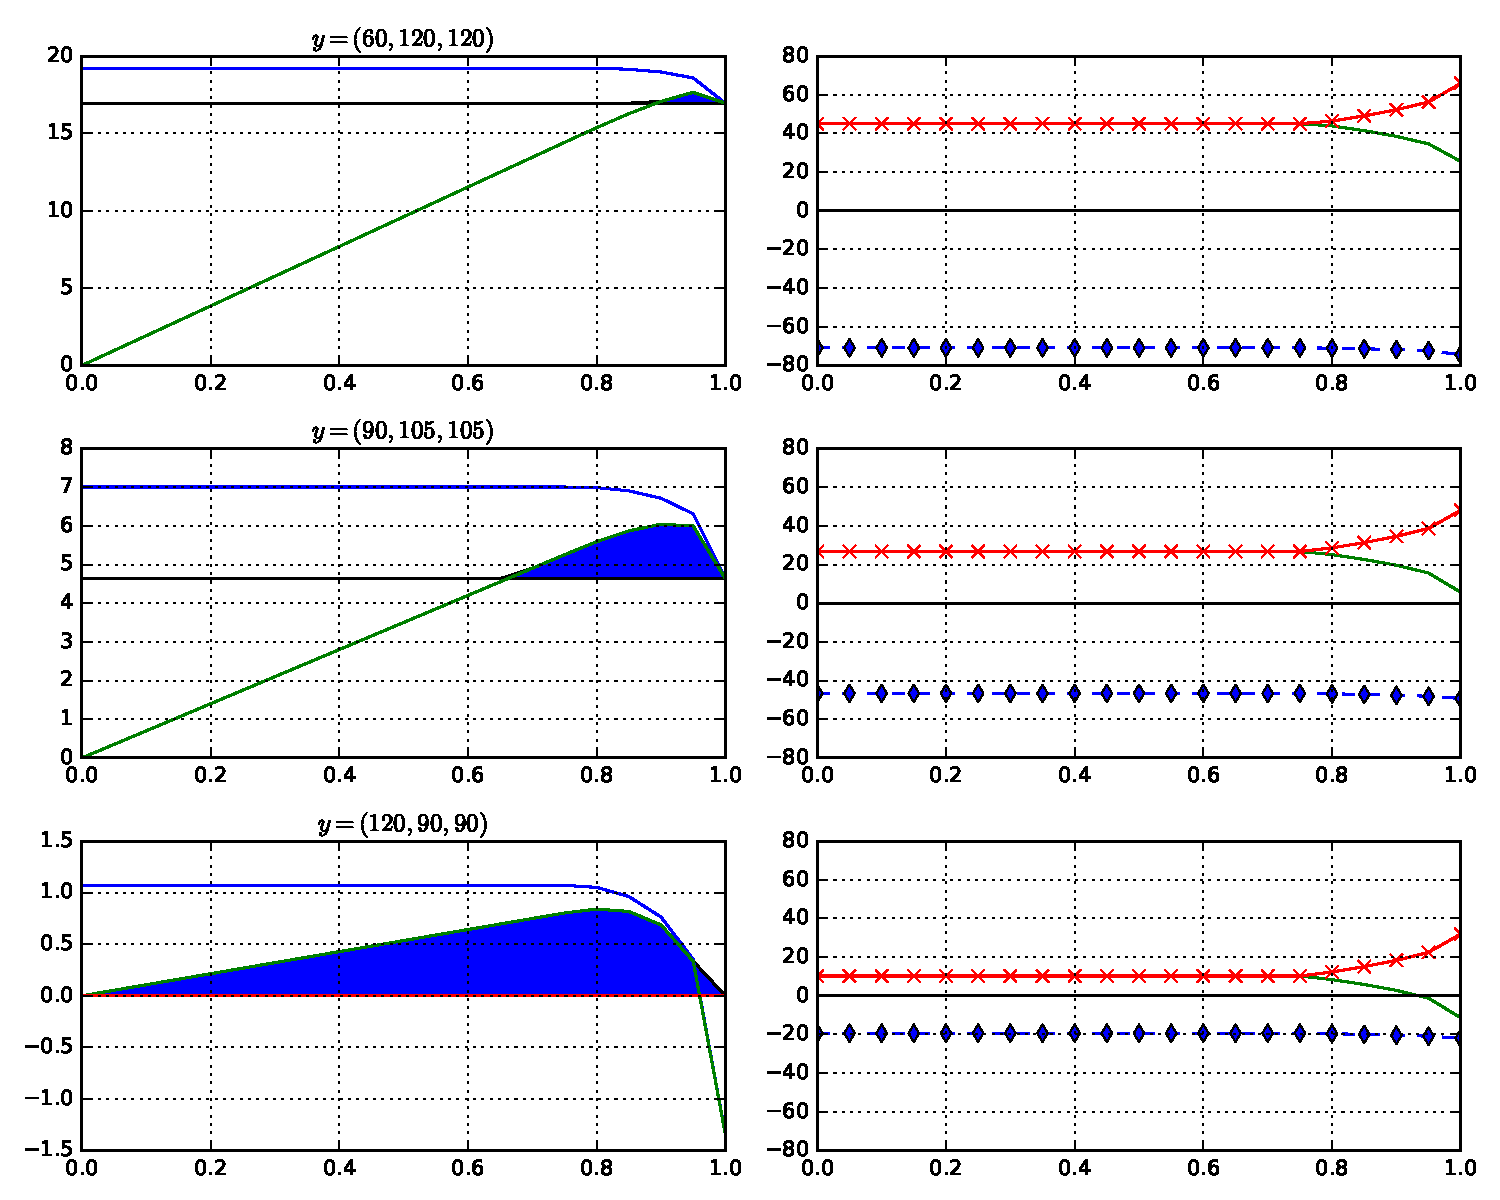
\includegraphics[width=\textwidth]{fig_nonprofits.pdf}
\caption{\label{fig:nonprofit}Choice of non-profit status and initial endowment
income}
\end{figure}


In Figure \ref{fig:nonprofit} we illustrate the case where non-pecuniary
costs to breaking a promise not to renegotiate fall with $\alpha$
according to $\eta(\alpha)=10(1-\alpha)$ and hence that the overall
cost to renegotiation varies with $\alpha$ according to $\kappa(\alpha)=10(1-\alpha)/\alpha$.
The plots depict captured profits that would be achieved at different
levels $\alpha$ starting from three different initial endowment streams.
These three streams - (60, 120, 120), (90, 105, 105) and (120, 90,
90) -- are equal in their present value of 300 but differ in terms
of period 0 income (with remaining income allocated equally across
period 1 and 2). The higher of the two curved lines represents `raw'
profits $\Pi_{0}(C_{0}^{m,\alpha};Y)$ and the lower curve captured
profits $\alpha\Pi_{0}(C_{0}^{m,\alpha};Y)$. A horizontal line has
been drawn in to indicate the level of profits $\Pi_{0}(C_{0}^{m,1};Y)$
captured by a pure for-profit ($\alpha=1$). Consider the top panel
where the customer has initial income $(60,120,120)$. As this type
of customer wants to borrow heavily in period 0 profits to the bank
are large, even in the case of renegotiation proof contracts. Adopting
non-profit status by lowering $\alpha$ confers no profit gain however:
the cost of lowering alpha (giving up a share of already high profits)
is not compensated for by the gains from being able to credibly commit
to a smoother contract. However at $(90,105,105)$ the tradeoff is
different and profits can be increased. In the picture any non-profit
with an $\alpha$ between approximately 0.7 and less than one captures
more profits than a pure for-profit. Finally for customers with an
endowment $(120,90,90)$ are already fairly close to their preferred
consumption stream so the profits to be captured even under full commitment
are not that large. Indeed in this case a pure for-profit cannot earn
positive profits. Here the cost of adopting non-profit status is low
compared to the gains, and we the simulation reveal that any non-profit
status firm captures more profits than a pure for-profit, and maximum
captured profits are achieved at around $\alpha=0.7$.

We conclude this section with a note on the nature of profit-capture
restrictions faced by a nonprofit. Our assumption that the firm can
capture a fixed fraction of raw profits was useful for exposition
but is perhaps not realistic, and is not necessary for our results.
We might imagine that, at low levels of profits, the nonprofit can
capture most of the profits, and that as profits rise so do the restrictions
on the firm's ability to capture them. In other words, a nonprofit
captures $f\left(\Pi\right)$ of profits, where $f\left(0\right)=0$,
$0<f'\left(\Pi\right)<1$, and $f''\left(\Pi\right)<0.$ In such cases,
we can again clearly see how non-profit status could be attractive
to the firm: the concavity of $f$ can leave the enjoyment of profits
relatively unaffected while significantly loosening the no-renegotiation
constraint (since renegotiation would raise profits further, and since
$f$ is concave, these additional profits would count for little).


\subsection{Competition}


\subsubsection{Exclusive contracts}

Consider what would happen in the competitive market situation now
if contracts can be assumed to remain exclusive, so that any new surplus
in the event of a renegotiation between the bank and the period 1
self goes to the bank (this grants the bank monopoly power in period
1). A firm of type $\alpha$ will be led to offer contract terms to
solve
\begin{align}
\underset{C_{0}}{max} & U_{0}\left(C_{0}\right)\nonumber \\
s.t. & \alpha\Pi_{0}(C_{0};Y_{0})\geq0\\
 & \Pi_{0}(C_{1}^{r}(C_{1});C_{1})\leq\kappa(\alpha)
\end{align}


Here, as before, $\kappa(\alpha)=\frac{\eta(\alpha)}{\alpha}$, captures
the idea that the principals of a firm that adopts non-profit status
commit themselves to capturing a smaller share of raw profits and
may also suffer greater direct disutility from breaking promises to
customers. Let the contract that solves this program be denoted $C_{0}^{c,e,np}$
(`competition, exclusive, nonprofit').

Consider first a field where all firms start as pure for-profits ($\alpha=1$).
If the no-renegotiation constraint binds, consumer welfare must be
lower than that when the firms can commit to not renegotiate since
an additional constraint is imposed. Starting from this situation
consider now one firm's strategic choice of whether to adopt non-profit
status (i.e. to change its ownership and governance structures to
an $\alpha=\bar{\alpha}<1$ relaxing the no-renegotiation constraint.
One firm deviating into nonprofit status in this way can make positive
profits. So, if the borrowers are sophisticated hyperbolics, in equilibrium
all firms become nonprofit. As proven in the appendix, competition
will ensure however that in equilibrium the principals of all firms
are capturing zero profits.


\subsubsection{Non-Exclusive Contracts}

In the previous section, we had a setting with competition in period
0 but exclusive contracting and monopoly power in period 1. Now, assume
that exclusivity and period 1 monopoly power disappears. Firms can
compete to renegotiate each other's contracts in period 1. 

If there were only nonprofits in equilibrium, any one firm could make
positive profits by switching to for-profit status and undoing a rival
bank's contract in period 1. The advantages of undercutting other
firms' contracts outweigh the benefits of promising one's own clients
it will not renegotiate. As a result, equilibrium contracts will be
determined by for-profit firms, and consumers will be offered lower
commitment than from non-profit firms alone.\footnote{The same argument applies if banks can costlessly renegotiate other
bank's contracts.}
\begin{prop}
Consider any $\bar{\alpha}<1$ and a corresponding $\eta\left(\bar{\alpha}\right)=\kappa$.

(a) In a competitive banking market with exclusive contracts, all
active firms will be nonprofits (contracts will be offered for $U_{0}^{A}\leq\bar{U}^{np}$,
with $\bar{U}^{np}>\bar{U}$ as defined in Proposition 6).

(b) In a competitive banking market with non-exclusive contracts,
for-profits must exist in equilibrium (contracts will be offered for
$U_{0}^{A}\leq\bar{U}$, with $\bar{U}$ as defined in Proposition
2).
\end{prop}

\section{Discussion}


\subsection{Summary}

The model above formalizes the renegotiation problem faced by banks
that contract with hyperbolic discounters, and shows how the problem
is addressed in equilibrium contracts. Figure \ref{fig:Summary} summarizes
the key results of Sections 4-6. We show how contracts depend on relative
distances from the optimal autarky utility, $U_{0}^{*}$. The results,
taken together, generate some natural yet novel empirical predictions
that are in principle testable. 

\begin{figure}
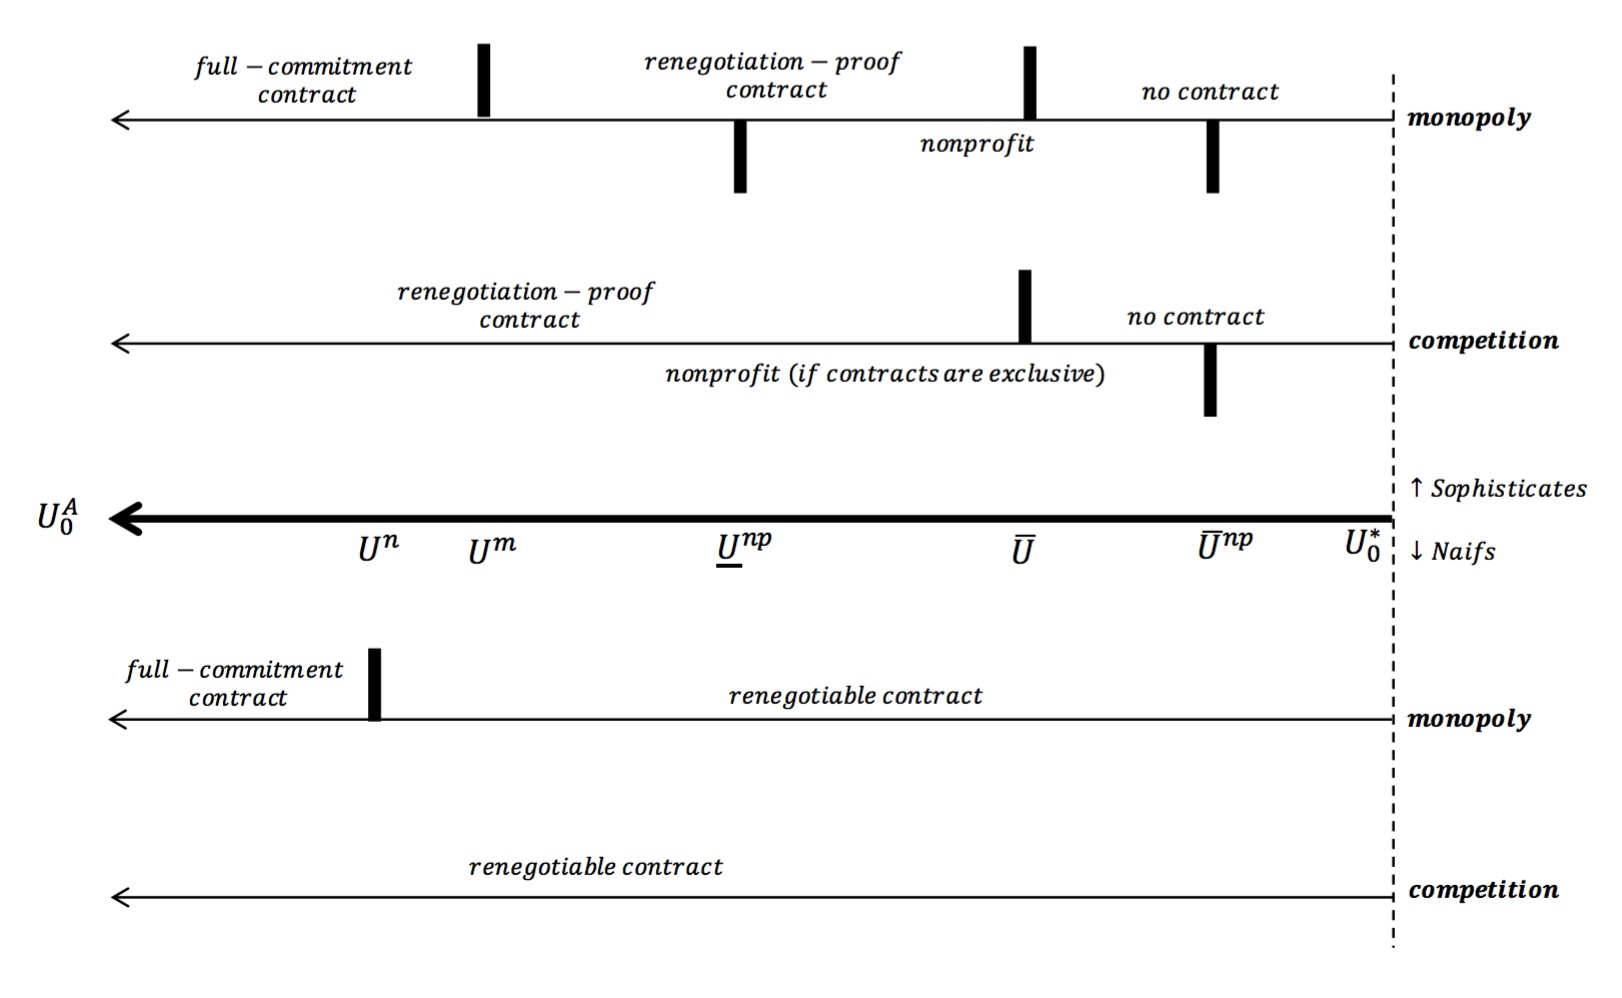
\includegraphics[scale=1.0]{fig_results}

\caption{\label{fig:Summary}Summary of results}
\end{figure}


We first discuss naive hyperbolic discounters. Under monopoly, contracts
will be subject to renegotiation if the consumer is close enough to
optimal autarky; if not, the full-commitment contract leaves the consumer
with so little consumption that there is no point renegotiating. The
parameter region in which contracts are renegotiated is relatively
large, and even includes cases where the sophisticate would be offered
a full-commitment contract. The renegotiable contract involves less
period-0 consumption that the full-commitment contract as this allows
the bank to exploit renegotiation possibilities most comprehensively.

Under competition, any contract will be renegotiated, even for consumers
whose autarky outcomes are very poor. This is because competitive
full-commitment contracts always leave consumers with relatively high
levels of future consumption. The implications for contract terms
are ambiguous.

Next, we turn to sophisticated hyperbolic discounters under monopoly.
If the consumer's smoothing needs are large (i.e. autarky utility
is low), full-commitment is feasible since the contract terms leave
little that is susceptible to renegotiation. If smoothing needs are
moderate, the consumer is offered a renegotiation-proof contract which
has a larger period-0 consumption than the full-commitment contract
(this serves to reduce the contract's susceptibility to renegotiation).
If smoothing needs are small, the consumer is better off in autarky
than in any contract that satisfies the renegotiation-proof constraint.
As a result of the problem of renegotiation, such consumers will not
be offered contracts.

Under competition, sophisticates will not be offered full-commitment
contracts. Since full-commitment would entail high consumption levels
in periods 1 and 2 regardless of autarky utility, the renegotiation-proofness
constraint must always bind. As under naivete, the implications for
contract terms are ambiguous.

Finally, we derive conditions under which banks will operate as nonprofits.
A monopoly will switch to a nonprofit if, as a for-profit its profits
were close to zero (above or below). In these cases, the bank is willing
to forgo some enjoyment of its profits in exchange for a loosened
renegotiation-proofness constraint. So, nonprofits will be able to
serve some consumers relatively closer to optimal autarky utility,
ones who would be unbanked under for-profit monopoly.

Under competition, banks should operate as nonprofits if contracts
are exclusive, as they can capture the surplus from improved contracts
possible under nonprofit status. If contracts are non-exclusive, no
bank can benefit from operating as a nonprofit, and for-profit banks
prevail.


\subsection{Additional Considerations}

Our model delivers predictions about how renegotiation concerns affect
commitment contracts, and about parameter regions in which these concerns
actually matter. In particular, we generate comparative statics over
autarky utilities. Autarky utility is not informative in isolation,
but in conjunction with total income serves as an indicator of the
extent of smoothing that remains to be provided by a bank. As we show,
contract terms depend in particular ways at different degrees of smoothing
needs.

The sizes of relevant parameter regions discussed above will vary
according to other parameter values such as the cost of renegotiation,
$\kappa$, and total income, $y$. For example, as $\kappa$ rises
there will be an expansion of the parameter region in which full commitment
survives. On the other hand, as $y$ rises, commitment in general
will be harder to sustain since contracts terms must allow for higher
consumption in periods 1 and 2.

While the focus of our paper is on contracts, a few observations on
welfare can be made. Under hyperbolic discounting, there is no obvious
notion of welfare, and for our purpose we take it to the discounted
utility of the period 0 self. Clearly, for sophisticated hyperbolic
discounters under monopoly, welfare remains constant regardless of
renegotiation concerns and bank governance--the consumer is always
left with autarky utility. Under competition, welfare is lower under
renegotiation-proof contracts relative to full-commitment (when the
constraint binds), and nonprofits serve to raise welfare.

Finally, recall that our model assumes contracts can only be initiated
in period 1. As a result, the consumer knows that the alternative
to a period-0 contract is autarky, and the bank knows that if a contract
isn't signed in period 0 there are no remaining opportunities to contract
with the consumer. This determines participation constraints for both
the consumer and the bank. The model could easily be extended to allow
for contracts that are initiated in period 1. While this would alter
participation constraints, the qualitative results of our model would
continue to hold.

Consider how participation constraints change if contracts could also
be initiated in period 1. For the consumer, the possibility of a period
1 contract could either tighten or loosen the participation constraint
in period 0 (if the period 1 contract further skews consumption away
from period 2, the constraint loosens; otherwise it tightens). For
the bank, the possibility of a period 1 contract must weakly tighten
its participation constraint. The problem can be analyzed in the same
way as in our original model, but the parameter values under which
a bank will switch from for-profit to nonprofit status will change.
For example, consider the monopolist bank. If, as a for-profit, period
0 profits are nearly 0, its decision about whether to switch to nonprofit
status becomes more complicated--it could turn into a nonprofit and
thereby earn higher profits in period 0, but it must also consider
the possibility of remaining a for-profit and simply offering a contract
in period 1 rather than in period 0.


\section{Conclusion}

The starting point for this paper is the observation that the solution
to any commitment problem must also address a renegotiation problem.
We show how the renegotiation problem affects different types of consumers
and how it changes contract terms in sometimes unexpected ways. In
this context, we also provide a rationalization of commercial nonprofits
in the absence of asymmetric information.

We argue that the model sheds some light on trends in microfinance,
payday lending, and mortgage lending. We hope this paper also offers
a framework that can be built upon. The incorporation of additional
`real-world' factors could improve our understanding of particular
institutions and generate empirically relevant comparative statics.
Examples of these include nondeterministic incomes, private and heterogenous
types, collateral and strategic default, and longer time horizons.

Finally, the differences between monopoly and competition open up
some new, potentially interesting questions. How does market structure
evolve and what are the implications for commitment? And through this
evolution might there emerge third parties to contracts between consumers
and banks that can more effectively enforce the commitment that is
sought after on both sides of the market?

\appendix

\section{Appendix: CRRA Derivations and Proofs}


\subsection{Full-Commitment}

For the monopolist bank that offers full-commitment, the solution
is determined by the first-order condition and the consumer's participation
constraint:
\begin{align}
C_{0}^{m,fc} & =\left(\left(\frac{U_{0}^{A}\left(1-\rho\right)}{1+2\beta^{\frac{1}{\rho}}}\right)^{\frac{1}{1-\rho}},\beta^{\frac{1}{\rho}}\left(\frac{U_{0}^{A}\left(1-\rho\right)}{1+2\beta^{\frac{1}{\rho}}}\right)^{\frac{1}{1-\rho}},\beta^{\frac{1}{\rho}}\left(\frac{U_{0}^{A}\left(1-\rho\right)}{1+2\beta^{\frac{1}{\rho}}}\right)^{\frac{1}{1-\rho}}\right)\label{eq:c-mf}\\
\Pi_{0}\left(C_{0}^{m,fc};Y_{0}\right) & =y-\left(U_{0}^{A}\left(1-\rho\right)\right)^{\frac{1}{1-\rho}}\left(1+2\beta^{\frac{1}{\rho}}\right)^{\frac{-\rho}{1-\rho}}\label{eq:pi-mf}
\end{align}


For the competitive banks that offer full-commitment, the solutions
is determined by the first-order condition and the bank's participation
constraint:
\begin{equation}
C_{0}^{c,fc}=\left(\frac{y}{1+2\beta^{\frac{1}{\rho}}},\frac{\beta^{\frac{1}{\rho}}y}{1+2\beta^{\frac{1}{\rho}}},\frac{\beta^{\frac{1}{\rho}}y}{1+2\beta^{\frac{1}{\rho}}}\right)\label{eq:c-cf}
\end{equation}



\subsection{Renegotiation}

Given an existing contract $C_{1}$, a monopolist bank that renegotiates
in period 1 will offer the following new contract:
\begin{equation}
C_{1}^{r}\left(C_{1}\right)=\left(\left(\frac{c_{1}^{1-\rho}+\beta c_{2}^{1-\rho}}{1+\beta^{\frac{1}{\rho}}}\right)^{\frac{1}{1-\rho}},\beta^{\frac{1}{\rho}}\left(\frac{c_{1}^{1-\rho}+\beta c_{2}^{1-\rho}}{1+\beta^{\frac{1}{\rho}}}\right)^{\frac{1}{1-\rho}}\right)\label{eq:c-r}
\end{equation}


The corresponding profit gains from renegotiation are:
\begin{equation}
\Pi_{1}\left(C_{1}^{r}\left(C_{1}\right);C_{1}\right)=\left(c_{1}+c_{2}\right)-\left(c_{1}^{1-\rho}+\beta c_{2}^{1-\rho}\right)^{\frac{1}{1-\rho}}\left(1+\beta^{\frac{1}{\rho}}\right)^{\frac{-\rho}{1-\rho}}\label{eq:pi-r}
\end{equation}


An alternate way to restate the above is the following: Let $s$ and
$\alpha$ be defined such that $c_{1}=\alpha s$ and $c_{2}=\left(1-\alpha\right)s$.
Then:
\begin{equation}
C_{1}^{r}\left(C_{1}\right)=\left(s\left(\frac{\alpha^{1-\rho}+\beta\left(1-\alpha\right)^{1-\rho}}{1+\beta^{\frac{1}{\rho}}}\right)^{\frac{1}{1-\rho}},s\beta^{\frac{1}{\rho}}\left(\frac{\alpha^{1-\rho}+\beta\left(1-\alpha\right)^{1-\rho}}{1+\beta^{\frac{1}{\rho}}}\right)^{\frac{1}{1-\rho}}\right)\label{eq:c-r-alpha}
\end{equation}


Profit gains from renegotiation become:
\begin{equation}
\Pi_{1}\left(C_{1}^{r}\left(C_{1}\right);C_{1}\right)=\left(s\right)\left(1-\left(\alpha^{1-\rho}+\beta\left(1-\alpha\right)^{1-\rho}\right)^{\frac{1}{1-\rho}}\left(1+\beta^{\frac{1}{\rho}}\right)^{\frac{-\rho}{1-\rho}}\right)\label{eq:renegotiation-profits}
\end{equation}


By construction, profits from renegotiation are strictly positive
(and increasing in $s$), except in the special case where $C_{1}$
is optimal from period 1's perspective ($\left(1-\alpha\right)=\beta^{\frac{1}{\rho}}\alpha$),
in which case they are $0$. It can also easily be confirmed that
profits from renegotiation fall in $\alpha$ as long as the allocation
is such that period 1 would like a larger $\alpha$ than the current
contract offers.

\textbf{\textit{Proof of Proposition 1:}} (a) In any full-commitment
contract, $\alpha=\frac{1}{2}$. Inserting this into (\ref{eq:renegotiation-profits}),
the following must be satisfied for a full-commitment contract to
survive:
\begin{equation}
k\geq s\left(1-\frac{1}{2}\left(1-\beta\right)^{\frac{1}{1-\rho}}\left(1+\beta^{\frac{1}{\rho}}\right)^{\frac{-\rho}{1-\rho}}\right)\label{eq:max-kappa-part}
\end{equation}
Substituting for $s$ from the competitive full-commitment contract,
we can rewrite the above condition as:
\begin{equation}
k\geq\frac{2\beta^{\frac{1}{\rho}}y}{1+2\beta^{\frac{1}{\rho}}}\left(1-\frac{1}{2}\left(1-\beta\right)^{\frac{1}{1-\rho}}\left(1+\beta^{\frac{1}{\rho}}\right)^{\frac{-\rho}{1-\rho}}\right)\equiv\bar{\kappa}\label{eq:max-kappa}
\end{equation}
Since in any full-commitment contract (monopoly and competition),
$s$ will be no larger than $\frac{2\beta^{\frac{1}{\rho}}y}{1+2\beta^{\frac{1}{\rho}}}$,
no full-commitment contract will be renegotiated if $\kappa\geq\bar{\kappa}$.

(c) If $\kappa<\bar{\kappa}$, condition \ref{eq:max-kappa} fails,
so the competitive full-commitment contract cannot survive. 

(b) The monopolist full-commitment contract will not survive if $s$
is sufficiently large. Since $s^{m,fc}$ is exponentially increasing
in $U_{0}^{A}$, there must be some $U^{m}$ such that the contract
will not survive if and only if $U_{0}^{A}>U^{m}$. Since the contract
cannot survive at $U_{0}^{*}$ (here, the contract is identical to
the competitive contract) , $U^{m}<U_{0}^{*}$. $\Square$


\subsection{Renegotiation-Proof Contracts}


\subsubsection{Sophisticated Hyperbolic Discounters}

When the renegotiation-proofness constraint binds, consumption in
periods 1 and 2 must satisfy:
\begin{equation}
\left(s\right)\left(1-\left(\alpha^{1-\rho}-\beta\left(1-\alpha\right)^{1-\rho}\right)^{\frac{1}{1-\rho}}\left(1+\beta^{\frac{1}{\rho}}\right)^{\frac{-\rho}{1-\rho}}\right)=\kappa\label{eq:rp-constraint}
\end{equation}


For any $s$, there may be two values of $\alpha$ that satisfy the
constraint with equality--one with too little consumption relative
to period 1's optimal, one with too much consumption relative to period
1's optimal. The relevant value for us is the first. This defines
a continuous function $\alpha\left(s\right)$.
\begin{equation}
\alpha\left(s\right)=min\left\{ \alpha:\left(s\right)\left(1-\left(\alpha^{1-\rho}+\beta\left(1-\alpha\right)^{1-\rho}\right)^{\frac{1}{1-\rho}}\left(1+\beta^{\frac{1}{\rho}}\right)^{\frac{-\rho}{1-\rho}}\right)=\kappa\right\} \label{eq:alpha}
\end{equation}


As $s$ rises, to continue satisfying the constraint we must have
$\alpha\left(s\right)$ rising too (if fractions stayed constant,
profits from renegotiation would rise).

We can also rewrite the first-order condition of the bank's maximization
problem using the new notation. For any $s$ and $\alpha$, let $V\left(s,\alpha\right)=u\left(\alpha s\right)+u\left(\left(1-\alpha\right)s\right)$.
This is the discounted utility over periods 1 and 2, from period 0's
perspective. The solution, $C_{0}=$$\left(c_{0},\alpha s,\left(1-\alpha\right)s\right)$,
must satisfy:
\begin{equation}
\frac{du\left(c_{0}\right)}{dc_{0}}=\beta\frac{dV\left(s,\alpha\right)}{ds}\label{eq:du-dv}
\end{equation}


In other words, at the profit-maximizing contract the marginal dollar
should be equally valuable whether consumed immediately or distributed
across future periods.

\textbf{\textit{Proof of Proposition 2:}} (a) Since the profit-maximizing
contract was uniquely determined, and since it does not satisfy the
renegotiation-proofness constraint, the renegotiation-proof contract
must yield lower profits than the full-commitment contract does.

(b) Clearly, $\Pi_{0}\left(C_{0}^{m,rp};Y_{0}\right)$ falls strictly
in $U_{0}^{A}$ (if autarky utility falls, the bank can always do
better, at least by simply lowering $c_{0}$). Since at $U_{0}^{A}=U^{m}$,
$\Pi_{0}\left(C_{0}^{m,rp};Y_{0}\right)=\Pi_{0}\left(C_{0}^{m,fc};Y_{0}\right)>0$
and at $U_{0}^{A}=U^{*}$, $\Pi_{0}\left(C_{0}^{m,rp};Y_{0}\right)<\Pi_{0}\left(C_{0}^{m,fc};Y_{0}\right)=0$,
there must be some intermediate autarky utility above which the bank's
maximized profits will be negative.

(c) consider any $c_{0}\leq c_{0}^{m,fc}$ and $s$ such that $U_{0}\left(c_{0},\frac{s}{2},\frac{s}{2}\right)=U_{0}^{A}$.
We can find the corresponding $\bar{s}$ that, while satisfying the
participation constraint, gives the same utility from period 0's perspective: 

\begin{align}
V\left(s,\frac{1}{2}\right) & =\bar{V}\left(\bar{s},\alpha\left(\bar{s}\right)\right)\label{eq:v=00003Dvbar1}\\
\Rightarrow2\frac{\left(\frac{1}{2}s\right)^{1-\rho}}{1-\rho} & =\frac{\left(\alpha\left(\bar{s}\right)\bar{s}\right)^{1-\rho}}{1-\rho}+\frac{\left(\left(1-\alpha\left(\bar{s}\right)\right)\bar{s}\right)^{1-\rho}}{1-\rho}\label{eq:v-vbar2}\\
\Rightarrow\bar{s} & =s\left(\frac{2\left(\frac{1}{2}\right)^{1-\rho}}{\alpha\left(\bar{s}\right)^{1-\rho}+\left(1-\alpha\left(\bar{s}\right)\right)^{1-\rho}}\right)^{\frac{1}{1-\rho}}\label{eq:v-vbar3}
\end{align}


From this, we get the following inequality:
\begin{align}
\frac{dV\left(\bar{s},\alpha\left(\bar{s}\right)\right)}{ds} & =\bar{s}^{-\rho}\left(\alpha\left(\bar{s}\right)^{1-\rho}+\left(1-\alpha\left(s\right)\right)^{1-\rho}\right)+\frac{d\alpha\left(\bar{s}\right)}{ds}\bar{s}^{1-\rho}\left(\alpha\left(\bar{s}\right)^{-\rho}-\left(1-\alpha\right)^{-\rho}\right)\label{eq:dv-ds1}\\
 & <\bar{s}^{-\rho}\left(\alpha\left(\bar{s}\right)^{1-\rho}+\left(1-\alpha\left(s\right)\right)^{1-\rho}\right)\label{eq:dv-ds2}\\
 & =s^{-\rho}\left(2\left(\frac{1}{2}\right)^{1-\rho}\right)\left(\frac{2\left(\frac{1}{2}\right)^{1-\rho}}{\alpha\left(\bar{s}\right)^{1-\rho}+\left(1-\alpha\left(\bar{s}\right)\right)^{1-\rho}}\right)^{\frac{-1}{1-\rho}}\label{eq:dv-ds3}\\
 & <s^{-\rho}\left(2\left(\frac{1}{2}\right)^{1-\rho}\right)=\frac{dV\left(s,\frac{1}{2}\right)}{ds}\label{eq:dv-ds4}
\end{align}


The first line above splits the effect of $s$ on $V$ into two--the
first term represents the change in utility holding $\alpha$ constant,
and the second term represents the (negative) effect of the further
skewing of consumption that results from a rise in $s$. The final
inequality follows from the fact that, since $\bar{s}>s^{m,fc}$,
the renegotiation constraint must bind so that $\alpha\left(\bar{s}\right)>\frac{1}{2}$.
Finally, the following inequality holds:
\begin{align}
\frac{du\left(c_{0}\right)}{dc_{0}} & \geq\frac{du\left(c_{0}^{m,fc}\right)}{dc_{0}}=\beta\frac{dV\left(s^{m,fc},\frac{1}{2}\right)}{ds}\label{eq:dudc-dvds1}\\
 & \geq\beta\frac{dV\left(s,\frac{1}{2}\right)}{ds}>\beta\frac{dV\left(\bar{s},\alpha\left(\bar{s}\right)\right)}{ds}\label{eq:dudc-dvds2}
\end{align}


We have shown that at any $c_{0}\leq c_{0}^{m,fc}$, for a contract
that satisfies the renegotiation-proofness constraint, the marginal
utility of period 0 consumption will be higher than the discounted
marginal utility of future consumption, so the bank could earn strictly
higher profits by raising $c_{0}$ and lowering $s$ further. Therefore,
in the renegotiation-proof contract, $c_{0}^{m,rp}>c_{0}^{m,fc}$.
$\Square$

\textbf{\emph{Proof of Proposition 3:}} (a) We know that $U_{0}\left(C_{0}^{c,fc}\right)=U_{0}^{*}$.
By assumption, since the renegotiation-proofness constraint is binding,
the renegotiation-proof contract cannot offer the optimal consumption
path. Therefore $U_{0}\left(C_{0}^{c,rp}\right)<U_{0}\left(C_{0}^{c,fc}\right)$.

(b) Consider $\bar{U}$, as constructed in Proposition 2. If $U_{0}^{A}>\bar{U}$,
it is impossible to construct a contract that earns nonnegative profits
and gives the consumer at least autarky utility. Therefore, any contract
that earns zero profits would give the period 0 consumer less than
autarky utility. (As an aside, observe that $\bar{U}=U_{0}\left(C_{0}^{c,rp}\right)$.)

(c) At the full-commitment contract:
\begin{equation}
\frac{du\left(c_{0}^{c,fc}\right)}{dc}=\beta\frac{dV\left(s^{c,fc},\frac{1}{2}\right)}{ds}=\left(s^{c,fc}\right)^{-\rho}\left(2\left(\frac{1}{2}\right)^{1-\rho}\right)
\end{equation}
Consider a renegotiation-proof contract with $c_{0}=c_{0}^{c,fc}$.
To keep bank profits zero, this contract would also have $s=s^{c,fc}$.
But in the renegotiation-proof contract, $s$ must be divided according
to the fraction $\alpha\left(s^{c,fc}\right)$. So:
\begin{align}
\frac{dV\left(s^{c,fc},\alpha\left(s^{c,fc}\right)\right)}{ds} & =\left(s^{c,fc}\right)^{-\rho}\left(\alpha\left(s^{c,fc}\right)^{1-\rho}+\left(1-\alpha\left(s^{c,fc}\right)\right)^{1-\rho}\right)\nonumber \\
 & +\frac{d\alpha\left(s^{c,fc}\right)}{ds}\left(s^{c,fc}\right)^{1-\rho}\left(\alpha\left(s^{c,fc}\right)^{-\rho}-\left(1-\alpha\left(s^{c,fc}\right)\right)^{-\rho}\right)\label{eq:dv-ds-comp}
\end{align}
The first term--the direct effect of a change in $s$--is weakly less
than $\frac{dV\left(s^{c,fc},\frac{1}{2}\right)}{ds}$ if $\rho\leq1$
and strictly greater if $\rho>1$. The second term--the component
of $\frac{dV}{ds}$ that is driven by the change in $\alpha$--is
strictly negative. Therefore, if $\rho<1$, $\frac{dV\left(s^{c,fc},\alpha\left(s^{c,fc}\right)\right)}{ds}<\frac{dV\left(s^{c,fc},\frac{1}{2}\right)}{ds}=\frac{du\left(c_{0}^{c,fc}\right)}{dc}$,
so the renegotiation-proof contract must satisfy $c_{0}^{c,rp}>c_{0}^{c,fc}$.

Next, we consider the case when $\rho>1$. We can make the following
observations about $\alpha\left(s\right)$. First, $\underset{\kappa\rightarrow0}{lim}\alpha\left(s\right)=\frac{\beta^{\frac{-1}{\rho}}}{1+\beta^{\frac{-1}{\rho}}}$
(this follows from the fact that at $\kappa=0$, the contract must
satisfy $u'\left(c_{1}\right)=\beta u'\left(c_{2}\right)$). Second,
implicitly differentiating equation \ref{eq:alpha} with respect to
$s$, and combining it with the previous limit result, we get $\underset{\kappa\rightarrow0}{lim}\frac{d\alpha\left(s\right)}{ds}=0$.
Therefore, if $\rho>1$ and $\kappa$ is small enough, the second
term in Equation \ref{eq:dv-ds-comp} will be sufficiently small in
magnitude that $\frac{dV\left(s^{c,fc},\alpha\left(s^{c,fc}\right)\right)}{ds}>\frac{dV\left(s^{c,fc},\frac{1}{2}\right)}{ds}=\frac{du\left(c_{0}^{c,fc}\right)}{dc}$.
In this case, the renegotiation-proof contract must satisfy $c_{0}^{c,rp}<c_{0}^{c,fc}$.
$\Square$

If $\kappa=0$, the renegotiation-proof contracts can be explicitly
derived since in any contract it must be true that $c_{2}=\beta^{\frac{1}{\rho}}c_{1}$.
Solving the respective maximization problems, we get the following
equilibrium contracts for monopoly and competition, respectively:
\begin{align}
C_{0}^{m,rp}= & \left(\left(\frac{U_{0}^{A}\left(1-\rho\right)}{1+\beta^{\frac{1}{\rho}}\left(\frac{\left(1+\beta^{\frac{1-\rho}{\rho}}\right)^{\frac{1}{\rho}}}{\left(1+\beta^{\frac{1}{\rho}}\right)^{\frac{1-\rho}{\rho}}}\right)}\right)^{\frac{1}{1-\rho}},\left(\frac{\beta+\beta^{\frac{1}{\rho}}}{1+\beta^{\frac{1}{\rho}}}\right)^{\frac{1}{\rho}}c_{0}^{m,rp},\beta^{\frac{1}{\rho}}\left(\frac{\beta+\beta^{\frac{1}{\rho}}}{1+\beta^{\frac{1}{\rho}}}\right)^{\frac{1}{\rho}}c_{0}^{m,rp}\right)\label{eq:zerokappa-monop}\\
C_{0}^{c,rp}= & \left(\frac{y}{1+\beta+\beta^{\frac{1}{\rho}}},\left(\frac{\beta+\beta^{\frac{1}{\rho}}}{1+\beta^{\frac{1}{\rho}}}\right)c_{0}^{c,rp},\beta^{\frac{1}{\rho}}\left(\frac{\beta+\beta^{\frac{1}{\rho}}}{1+\beta^{\frac{1}{\rho}}}\right)c_{0}^{c,rp}\right)\label{eq:zerokappa-comp}
\end{align}


It can easily be established that $c_{0}^{m,rp}>c_{0}^{m,fc}$, $c_{0}^{c,rp}>c_{0}^{m,fc}$
if $\rho>1$, and $c_{0}^{c,rp}<c_{0}^{m,fc}$ if $\rho<1$.


\subsubsection{Naive Hyperbolic Discounters}

Suppose the monopolist intends to renegotiate the contract. The maximization
problem, combined with the expression for $C_{1}^{r}\left(C_{1}\right)$
(\ref{eq:c-r-alpha}), simplifies to:

\begin{align}
\underset{c_{0},c_{1},c_{2}}{max} & y-c_{0}-\frac{\left(c_{1}^{1-\rho}+\beta c_{2}^{1-\rho}\right)^{\frac{1}{1-\rho}}}{\left(1+\beta^{\frac{1}{\rho}}\right)^{\frac{\rho}{1-\rho}}}-\kappa\\
s.t. & \frac{c_{0}^{1-\rho}}{1-\rho}+\beta\frac{c_{1}^{1-\rho}}{1-\rho}+\beta\frac{c_{2}^{1-\rho}}{1-\rho}\geq U_{0}^{A}
\end{align}


The partial derivatives of the resulting Lagrangian are:
\begin{align}
\frac{\partial\mathcal{L}}{\partial c_{0}} & =-1-\lambda c_{0}^{-\rho}\label{eq:L0}\\
\frac{\partial\mathcal{L}}{\partial c_{1}} & =c_{1}^{-\rho}\left[-\left(\frac{c_{1}^{1-\rho}+\beta c_{2}^{1-\rho}}{1+\beta^{\frac{1}{\rho}}}\right)^{\frac{\rho}{1-\rho}}-\lambda\beta\right]\label{eq:L1}\\
\frac{\partial\mathcal{L}}{\partial c_{2}} & =c_{2}^{-\rho}\left[-\beta\left(\frac{c_{1}^{1-\rho}+\beta c_{2}^{1-\rho}}{1+\beta^{\frac{1}{\rho}}}\right)^{\frac{\rho}{1-\rho}}-\lambda\beta\right]\label{eq:L2}
\end{align}


An interior solution, with $\frac{\partial\mathcal{L}}{\partial c_{1}}=0$
and $\frac{\partial\mathcal{L}}{\partial c_{2}}=0$ does not exist
since (on a $c_{1}-c_{2}$ plot, the two first-order conditions do
not intersect). If $\rho<1$, the Lagrangian is maximized at a corner
solution with $c_{1}=0$. If $\rho>1$, the Lagrangian is maximized
at the limit as $c_{2}$ approaches infinity. Using this, the maximization
problem can be re-solved. If $\rho<1$:
\begin{equation}
C_{0}^{m,n}=\left(\left(\frac{U_{0}^{A}\left(1-\rho\right)}{2+\beta^{\frac{1}{\rho}}}\right)^{\frac{1}{1-\rho}},0,\left(\frac{1+\beta^{\frac{1}{\rho}}}{\beta}\right)^{\frac{1}{1-\rho}}\left(\frac{U_{0}^{A}\left(1-\rho\right)}{2+\beta^{\frac{1}{\rho}}}\right)^{\frac{1}{1-\rho}}\right)\label{eq:naive-monopolist-contract1}
\end{equation}
If $\rho>1$, the solution is undefined, but in the limit is given
by:
\begin{equation}
C_{0}^{m,n}=\left(\left(\frac{U_{0}^{A}\left(1-\rho\right)}{1+\left(1+\beta^{\frac{1}{\rho}}\right)\beta^{\frac{1}{\rho}}}\right)^{\frac{1}{1-\rho}},\beta^{\frac{1}{\rho}}\left(1+\beta^{\frac{1}{\rho}}\right)^{\frac{1}{1-\rho}}\left(\frac{U_{0}^{A}\left(1-\rho\right)}{1+\left(1+\beta^{\frac{1}{\rho}}\right)\beta^{\frac{1}{\rho}}}\right)^{\frac{1}{1-\rho}},\infty\right)\label{eq:naive-monopolist-contract2}
\end{equation}


\textbf{\emph{Proof of Proposition 4:}} (a) At any autarky utility,
the monopolist could at least offer the full-commitment contract.

(b) The bank must choose between a renegotiation-proof contract and
a renegotiable contract (\ref{eq:naive-monopolist-contract1}, \ref{eq:naive-monopolist-contract2}).
By construction of $U^{m}$, the following must be true at any $U_{0}^{A}\geq U^{m}$:
\begin{equation}
\Pi_{0}\left(C_{0}^{m,rp};Y_{0}\right)\leq\Pi_{0}\left(C_{0}^{m,fc};Y_{0}\right)\leq\Pi_{0}\left(C_{0}^{m,fc};Y_{0}\right)+\Pi_{1}\left(C_{1}^{r}\left(C_{1}^{m,fc}\right);C_{1}^{m,fc}\right)-\kappa
\end{equation}


Since $C_{0}^{m,n}$ is uniquely determined and $C_{0}^{m,n}\neq C_{0}^{m,fc}$,
profits from the best renegotiable contract must be strictly higher
than profits from the renegotiation-proof contract at any $U_{0}^{A}\geq U^{m}$.

The following can be verified from the explicit derivations of $C_{0}^{m,fc}$
and $C_{0}^{m,n}$. First, if $U_{0}^{A}$ is sufficiently small,
$\Pi_{0}\left(C_{0}^{m,fc};Y_{0}\right)>\Pi\left(C_{0}^{m,n};Y_{0}\right)+\Pi_{1}\left(C_{1}^{r}\left(C_{1}^{m,n}\right);C_{1}^{m,n}\right)-\kappa$.
Second,
\begin{equation}
\frac{d}{dU_{0}^{A}}\Pi_{0}\left(C_{0}^{m,fc};Y_{0}\right)>\frac{d}{dU_{0}^{A}}\left[\Pi\left(C_{0}^{m,n};Y_{0}\right)+\Pi_{1}\left(C_{1}^{r}\left(C_{1}^{m,n}\right);C_{1}^{m,n}\right)-\kappa\right]
\end{equation}


It follows that there is some $U^{n}<U^{m}$ such that if $U_{0}^{A}\leq U^{n}$,
the naive agent will receive the monopoly full commitment contract,
which will be renegotiation-proof.

(c) This can be confirmed from the explicit formulations of $C_{0}^{m,fc}$
(\ref{eq:c-mf}) and $C_{0}^{m,n}$ (\ref{eq:naive-monopolist-contract1},
\ref{eq:naive-monopolist-contract2}). $\Square$

We now derive equilibrium contracts for naive consumers under perfect
competition. Suppose contracts are exclusive. Then, a contract that
is renegotiated satisfies:
\begin{align}
\underset{c_{0},c_{1},c_{2}}{max} & \frac{c_{0}^{1-\rho}}{1-\rho}+\beta\frac{c_{1}^{1-\rho}}{1-\rho}+\beta\frac{c_{2}^{1-\rho}}{1-\rho}\\
s.t. & y-c_{0}-\frac{\left(c_{1}^{1-\rho}+\beta c_{2}^{1-\rho}\right)^{\frac{1}{1-\rho}}}{\left(1+\beta^{\frac{1}{\rho}}\right)^{\frac{\rho}{1-\rho}}}-\kappa\geq0
\end{align}


The first-order conditions are the same as under monopoly (\ref{eq:L0},
\ref{eq:L1}, \ref{eq:L2}). Combining these with the zero-profit
constraint, we get the following solution. If $\rho<1$:
\begin{equation}
C_{0}^{c,n}=\left(\frac{y-\kappa}{2+\beta^{\frac{1}{\rho}}},0,\left(\frac{1+\beta^{\frac{1}{\rho}}}{\beta}\right)^{\frac{1}{1-\rho}}\left(\frac{y-\kappa}{2+\beta^{\frac{1}{\rho}}}\right)\right)\label{eq:naive-comp-contract1}
\end{equation}


If $\rho>1$, the solution is undefined, but in the limit is given
by:
\begin{equation}
C_{0}^{c,n}=\left(\frac{y-\kappa}{1+\beta^{\frac{1}{\rho}}\left(1+\beta^{\frac{1}{\rho}}\right)},\beta^{\frac{1}{\rho}}\left(1+\beta^{\frac{1}{\rho}}\right)^{\frac{1}{1-\rho}}\left(\frac{y-\kappa}{1+\beta^{\frac{1}{\rho}}\left(1+\beta^{\frac{1}{\rho}}\right)}\right),\infty\right)\label{eq:naive-comp-contract2}
\end{equation}


\textbf{\emph{Proof of Proposition 5:}} (a) Banks can at least offer
the consumer the full-commitment contract, so a contract is feasible
at any autarky utility. Since, from the consumer's perspective, any
renegotiation-proof contract is strictly dominated by the full-commitment
contract (which will be renegotiated), in equilibrium she will be
offered a contract that will be renegotiated.

(b) Under non-exclusive contracts, firms offering period 0 contracts
do not benefit from renegotiation (profits from renegotiation will
equal $\kappa$). So the equilibrium contract is identical to the
full-commitment contract.

(c) Suppose $\rho<1$. Comparing $C_{0}^{c,fc}$ (\ref{eq:c-cf})
to $C_{0}^{c,n}$ (\ref{eq:naive-comp-contract1}), it is clear that
$c_{0}^{c,n}<c_{0}^{c,fc}$. Suppose $\rho>1$. If $\kappa$ is small
enough, $c_{0}^{c,n}>c_{0}^{c,fc}$. $\Square$


\subsection{Nonprofits}
\begin{lem}
$\Pi_{0}\left(C_{0}^{m,rp};Y_{0}\right)$ and $\bar{\alpha}\Pi_{0}\left(C_{0}^{m,np};Y_{0}\right)$
are continuously decreasing in $U_{0}^{A}$.
\end{lem}
\textbf{\emph{Proof of Lemma 1: }}We prove the above for renegotiation-proof
contracts of for-profit banks. The same argument applies to nonprofit
banks. First, it is clear that profits are strictly decreasing in
$U_{0}^{A}$: If autarky utility drops from $U_{0}^{A}=U$ to $\bar{U_{0}^{A}=U}$,
at $\bar{U}$ the bank can always do better than offering the contract
it offered at $U$.

Next, we prove right-continuity at any $U_{0}^{A}=U$. Let the maximized
profits at $U$ be $\Pi_{0}\left(C_{0};Y_{0}\right)$, where $C_{0}=\left(c_{0},c_{1},c_{2}\right)$.
This contract must satisfy $U_{0}\left(C_{0}\right)=U$. For any $\bar{U}>U$,
profits must be lower, and bounded below by $\Pi_{0}\left(\bar{C}_{0};Y_{0}\right)$,
with the contract defined as $\bar{C}_{0}=\left(c_{0}+x,c_{1},c_{2}\right)$
where $x$ satisfies $U_{0}\left(\bar{C}_{0}\right)=\bar{U}$. Since
$\underset{\bar{U}\rightarrow U^{+}}{lim}\Pi_{0}\left(\bar{C}_{0};Y_{0}\right)=\Pi_{0}\left(C_{0};Y_{0}\right)$,
the profit function is right-continuous.

Finally, we prove left-continuity at at any $U_{0}^{A}=U$. For any
$\bar{U}<U$, denote maximized profits $\Pi_{0}\left(\bar{C}_{0};Y_{0}\right)$,
where $\bar{C}_{0}=\left(\bar{c}_{0},\bar{c}_{1},\bar{c}_{2}\right)$.
These contracts must satisfy $U_{0}\left(\bar{C}_{0}\right)=\bar{U}$.
At $U$, profits must be lower, and bounded below by $\Pi_{0}\left(C_{0};Y_{0}\right)$,
with the contract defined as $C_{0}=\left(\bar{c}_{0}+x,\bar{c}_{1},\bar{c}_{2}\right)$
where $x$ satisfies $U_{0}\left(C_{0}\right)=U$. Since $\underset{\bar{U}\rightarrow U^{-}}{lim}\Pi_{0}\left(\bar{C}_{0};Y_{0}\right)=\Pi_{0}\left(C_{0};Y_{0}\right)$,
the profit function is left-continuous. $\Square$

\textbf{\emph{Proof of Proposition 6: }}Let $\eta\left(\bar{\alpha}\right)=1$,
to minimize the attractiveness of the nonprofit. Consider $U_{0}^{A}=\bar{U}$.
Since the for-profit's renegotiation-proofness binds and leaves the
firm with zero profits, and since the non-profit's renegotiation-proofness
constraint is looser than the for-profit's, we know that $\bar{\alpha}\Pi\left(C_{0}^{m,np};Y_{0}\right)>0=\Pi\left(C_{0}^{m,rp};Y_{0}\right)$.
Since profits must be continuously decreasing in $U_{0}^{A}$, and
since $\bar{\alpha}\Pi\left(C_{0}^{m,np};Y_{0}\right)<\Pi\left(C_{0}^{m,rp},;Y\right)$
at $U_{0}^{A}=U^{m}$ (where the for-profit's renegotiation-proofness
constraint no longer binds) and $\bar{\alpha}\Pi\left(C_{0}^{m,np};Y_{0}\right)\leq0$
at $U_{0}^{A}=U_{0}^{*}$, there must exist autarky utility values
as described in the proposition statement such that, if $U_{0}^{A}>\underline{U}^{np}$
the bank strictly prefers to operate as a nonprofit relative to a
for-profit, and if $U_{0}^{A}\geq\bar{U}^{np}$ it weakly prefers
to not offer a contract. $\Square$

\textbf{\emph{Proof of Proposition 7: }}(a) Suppose all firms are
for-profit. There is some $\varepsilon_{1}$ and $\varepsilon_{2}$
satisfying $0<\varepsilon_{2}<\varepsilon_{1}$ and a corresponding
$\hat{C}_{0}=\left(c_{0}^{c,e,np},c_{1}^{c,e.np}-\varepsilon_{1},c_{2}^{c,e,np}+\varepsilon_{2}\right)$
such that $U_{0}\left(C_{0}^{c,e,np}\right)=U_{0}\left(\hat{C}_{0}\right)$
and $\Pi_{0}(C_{1}^{r}\left(\hat{C}_{1}\right);\hat{C}_{1})\leq\kappa(\mbox{\ensuremath{\bar{\alpha}}})$<$\kappa\left(1\right)$.
So, any firm can make positive profits by operating as a non-profit.
Therefore, in equilibrium, consumers will borrow only from non-profit
firms. Given the construction of $\bar{U}^{np}$, firms can make nonnegative
profits while satisfying the participation constraint only if $U_{0}^{A}\leq\bar{U}^{np}$.

(b) If all firms are nonprofit, an individual firm has a strict incentive
to switch to for-profit status, and make profits in period 1. Therefore,
there must be for-profits in equilibrium, and equilibrium contracts
will be constrained by their presence. $\Square$

\bibliographystyle{authordate1}
\bibliography{renegotiation}

\end{document}
